%%%%%%%%%%%%%%%%%%%%%%%%%%%%%%%%%%%%%%%%%
% Beamer Presentation
% LaTeX Template
% Version 1.0 (10/11/12)
%
% This template has been downloaded from:
% http://www.LaTeXTemplates.com
%
% License:
% CC BY-NC-SA 3.0 (http://creativecommons.org/licenses/by-nc-sa/3.0/)
%
%%%%%%%%%%%%%%%%%%%%%%%%%%%%%%%%%%%%%%%%%

%----------------------------------------------------------------------------------------
%	PACKAGES AND THEMES
%----------------------------------------------------------------------------------------

\documentclass[UTF8,aspectratio=169,12pt]{ctexbeamer}

\usepackage{hyperref}
\hypersetup{
	colorlinks=true,
	linkcolor=red,
	anchorcolor=blue,
	citecolor=green
}

\mode<presentation> {
	
	% The Beamer class comes with a number of default slide themes
	% which change the colors and layouts of slides. Below this is a list
	% of all the themes, uncomment each in turn to see what they look like.
	
	%\usetheme{default}
	%\usetheme{AnnArbor}
	%\usetheme{Antibes}
	%\usetheme{Bergen}
	%\usetheme{Berkeley}
	%\usetheme{Berlin}
	%\usetheme{Boadilla}
	%\usetheme{CambridgeUS}
	%\usetheme{Copenhagen}
	%\usetheme{Darmstadt}
	%\usetheme{Dresden}
	%\usetheme{Frankfurt}
	%\usetheme{Goettingen}
	%\usetheme{Hannover}
	%\usetheme{Ilmenau}
	%\usetheme{JuanLesPins}
	%\usetheme{Luebeck}
	\usetheme{Madrid}
	%\usetheme{Malmoe}
	%\usetheme{Marburg}
	%\usetheme{Montpellier}
	%\usetheme{PaloAlto}
	%\usetheme{Pittsburgh}
	%\usetheme{Rochester}
	%\usetheme{Singapore}
	%\usetheme{Szeged}
	%\usetheme{Warsaw}
	
	% As well as themes, the Beamer class has a number of color themes
	% for any slide theme. Uncomment each of these in turn to see how it
	% changes the colors of your current slide theme.
	
	%\usecolortheme{albatross}
	%\usecolortheme{beaver}
	%\usecolortheme{beetle}
	%\usecolortheme{crane}
	%\usecolortheme{dolphin}
	%\usecolortheme{dove}
	%\usecolortheme{fly}
	%\usecolortheme{lily}
	%\usecolortheme{orchid}
	%\usecolortheme{rose}
	%\usecolortheme{seagull}
	%\usecolortheme{seahorse}
	%\usecolortheme{whale}
	%\usecolortheme{wolverine}
	
	%\setbeamertemplate{footline} % To remove the footer line in all slides uncomment this line
	%\setbeamertemplate{footline}[page number] % To replace the footer line in all slides with a simple slide count uncomment this line
	
	%\setbeamertemplate{navigation symbols}{} % To remove the navigation symbols from the bottom of all slides uncomment this line
}

\usepackage{graphicx} % Allows including images
\graphicspath{{./figs/}}
\usepackage{booktabs} % Allows the use of \toprule, \midrule and \bottomrule in tables
\usepackage{longtable}
\usepackage{xcolor}
\usepackage{minted}
\usepackage{listings}
\lstset{numbers=left, %设置行号位置
	numberstyle=\tiny, %设置行号大小
	keywordstyle=\color{blue}, %设置关键字颜色
	commentstyle=\color[cmyk]{1,0,1,0}, %设置注释颜色
	frame=single, %设置边框格式
	escapeinside=``, %逃逸字符(1左面的键),用于显示中文
	%breaklines, %自动折行
	extendedchars=false, %解决代码跨页时,章节标题,页眉等汉字不显示的问题
	xleftmargin=2em,xrightmargin=2em, aboveskip=1em, %设置边距
	tabsize=4, %设置tab空格数
	showspaces=false %不显示空格
}
% Fonts
% \usepackage{libertine}
% \setmonofont{Courier}
%\setCJKsansfont[ItalicFont=Noto Serif CJK SC Black, BoldFont=Noto Sans CJK SC Black]{Noto Sans CJK SC}


%----------------------------------------------------------------------------------------
%	TITLE PAGE
%----------------------------------------------------------------------------------------

\title[第23讲]{第二十三讲 :Virtual Machine Monitor (Hypervisor)} % The short title appears at the bottom of every slide, the full title is only on the title page
\subtitle{第二节:How VMM works}
\author{向勇、陈渝、李国良} % Your name
\institute[清华大学] % Your institution as it will appear on the bottom of every slide, may be shorthand to save space
{
  清华大学计算机系 \\ % Your institution for the title page
  \medskip
  \textit{xyong,yuchen,liguoliang@tsinghua.edu.cn} % Your email address
}
\date{\today} % Date, can be changed to a custom date

\begin{document}

\begin{frame}
\titlepage % Print the title page as the first slide
\end{frame}

%\begin{frame}
%\frametitle{提纲} % Table of contents slide, comment this block out to remove it
%\tableofcontents % Throughout your presentation, if you choose to use \section{} and \subsection{} commands, these will automatically be printed on this slide as an overview of your presentation
%\end{frame}
%
%%----------------------------------------------------------------------------------------
%%	PRESENTATION SLIDES
%%----------------------------------------------------------------------------------------
%
%----------------------------------------------
\begin{frame}
\frametitle{提纲} % Table of contents slide, comment this block out to remove it
\tableofcontents % Throughout your presentation, if you choose to use \section{} and \subsection{} commands, these will automatically be printed on this slide as an overview of your presentation
\end{frame}
%%------------------------------------------------
\section{第二节:How VMM works} % Sections can be created in order to organize your presentation into discrete blocks, all sections and subsections are automatically printed in the table of contents as an overview of the talk
%%------------------------------------------------
\subsection{VMM Concept}
%-------------------------------------------------
% ### VMM Concept
% 
% * Host
% * Guest
% * vCPU
% * VM Entry/VM Exit
% 
% ![VMM-concept](/Users/xyong/Desktop/xyong-iMac/figs/VMM-concept.png)
% 
\begin{frame}
    \frametitle{VMM Concept}
    \begin{columns}
        \begin{column}{.3\textwidth}
            \begin{itemize}
                \item Host
                \item Guest
                \item vCPU
                \item VM Entry/VM Exit
            \end{itemize} 
        \end{column}
        \begin{column}{.7\textwidth}
            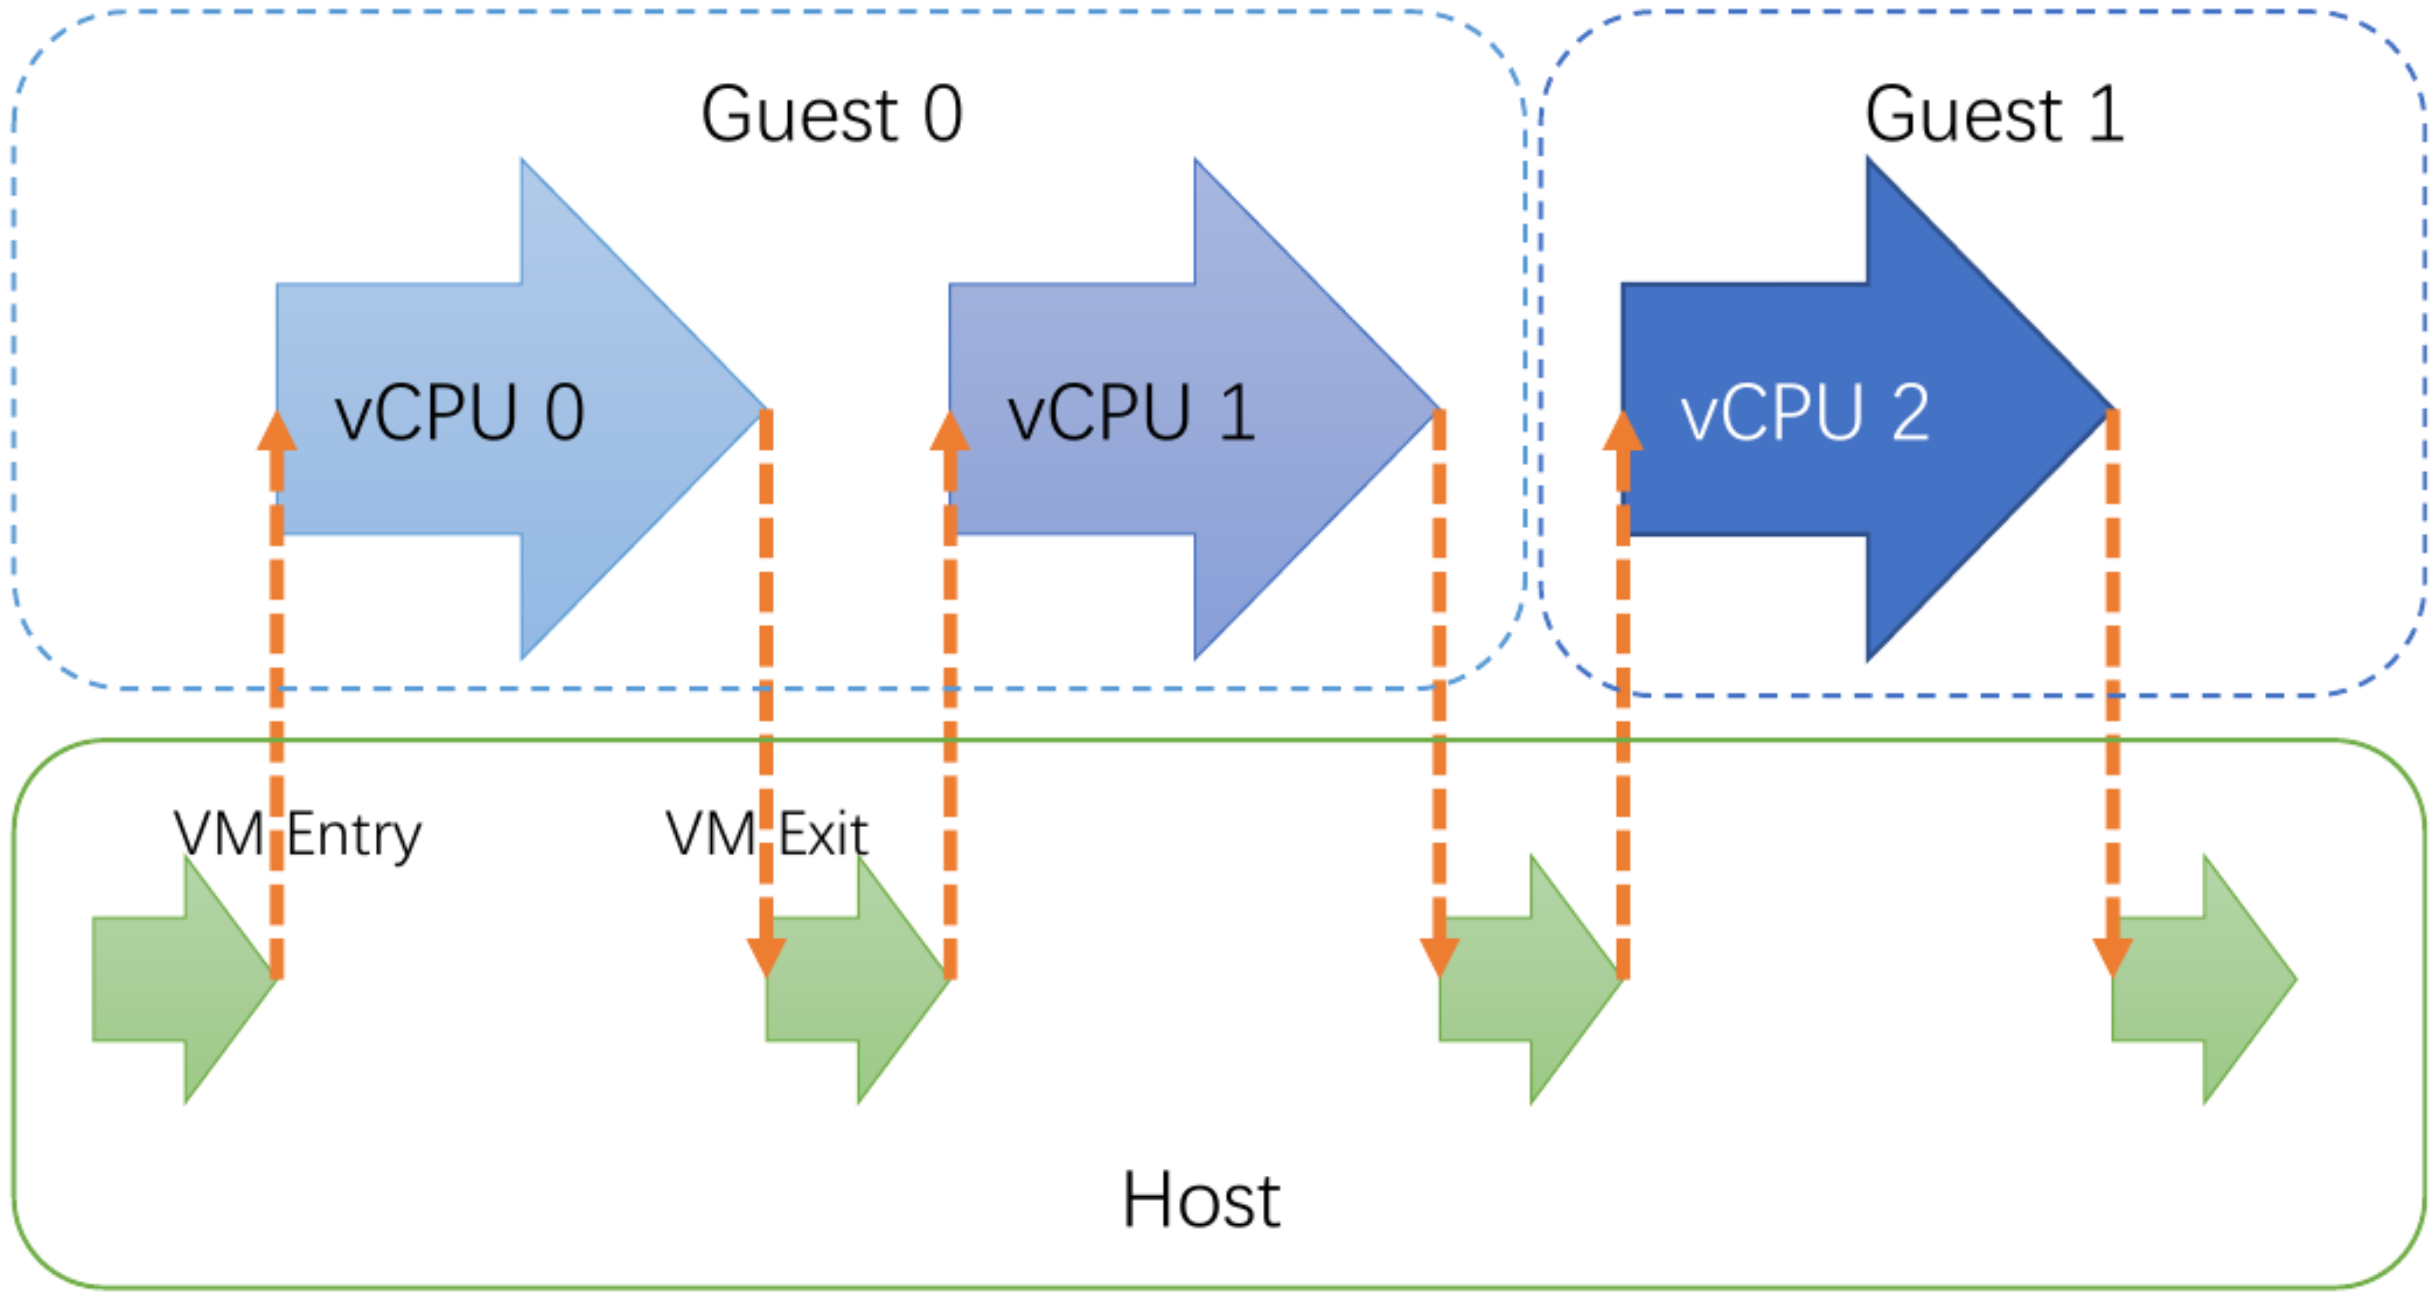
\includegraphics[width=1.\textwidth]{figs/VMM-concept.png}
        \end{column}
    \end{columns}

\end{frame}
%-------------------------------------------------
% ### Typer-1 & Type-0 VMM
% 
% ![type-1-2-VMM](/Users/xyong/Desktop/xyong-iMac/figs/type-1-2-VMM.png)
% 
\begin{frame}
    \frametitle{Typer-1 \& Type-0 VMM}
            \centering
            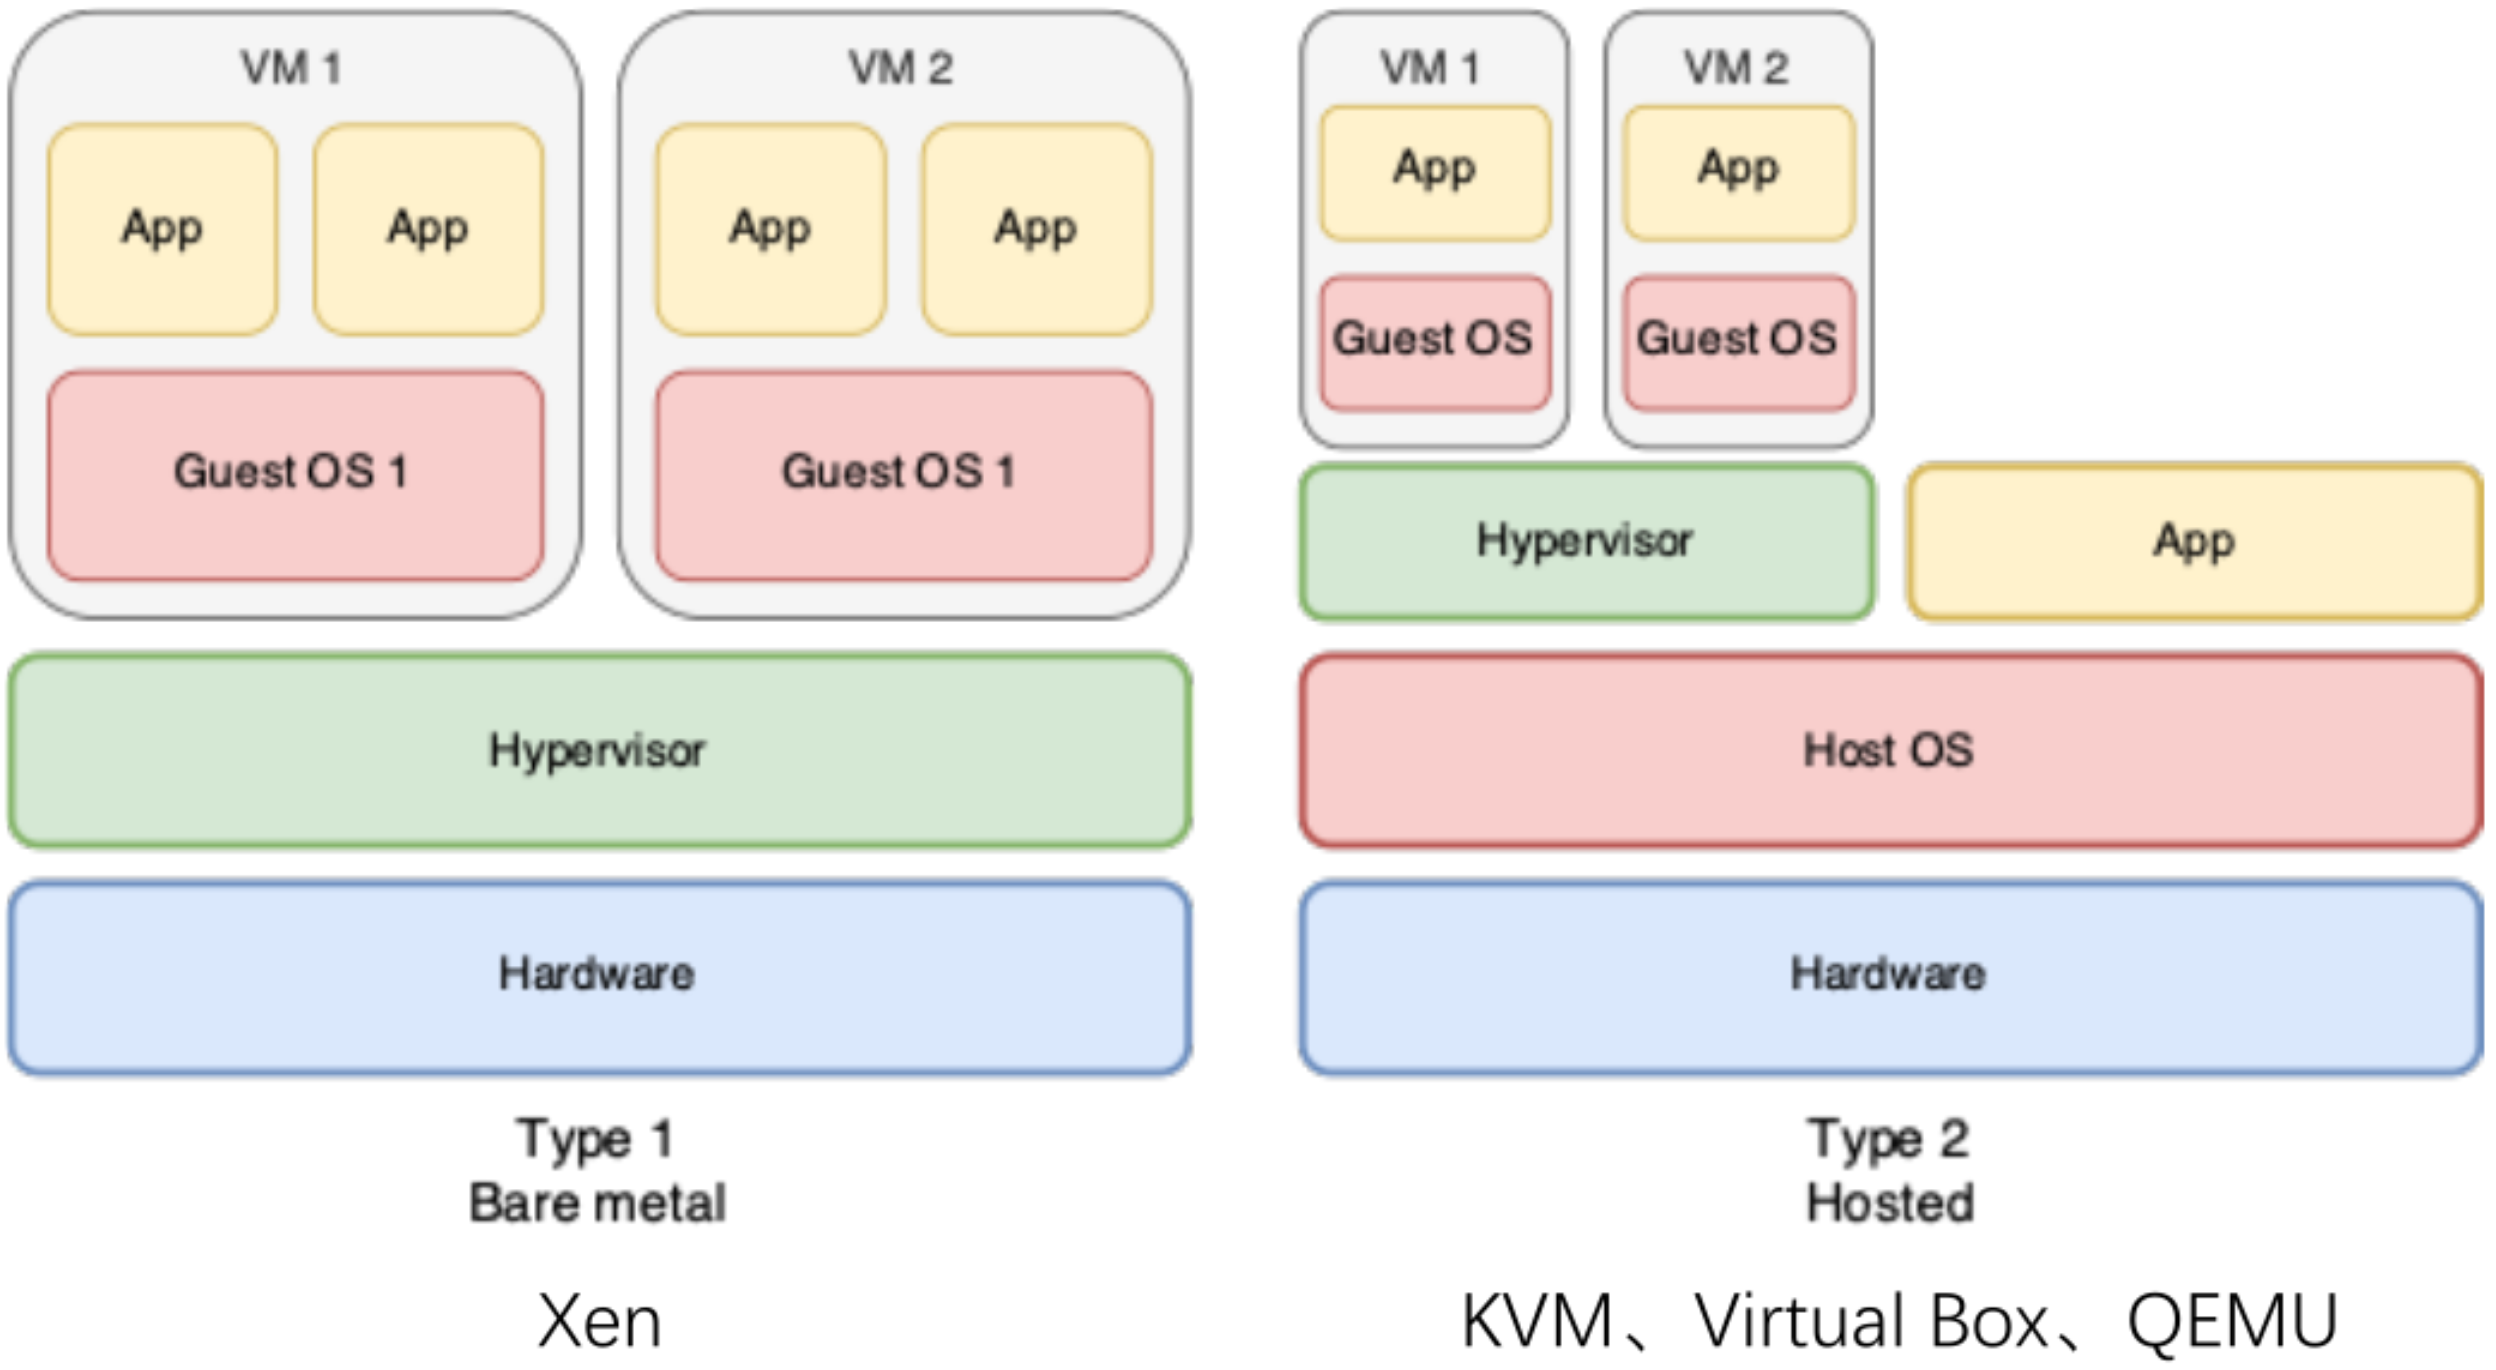
\includegraphics[width=0.85\textwidth]{figs/type-1-2-VMM.png}

\end{frame}
%-------------------------------------------------
% ### Type-1.5 VMM
% 
% ![type-1.5-VMM](/Users/xyong/Desktop/xyong-iMac/figs/type-1.5-VMM.png)
\begin{frame}
    \frametitle{Type-1.5 VMM}

            \centering
            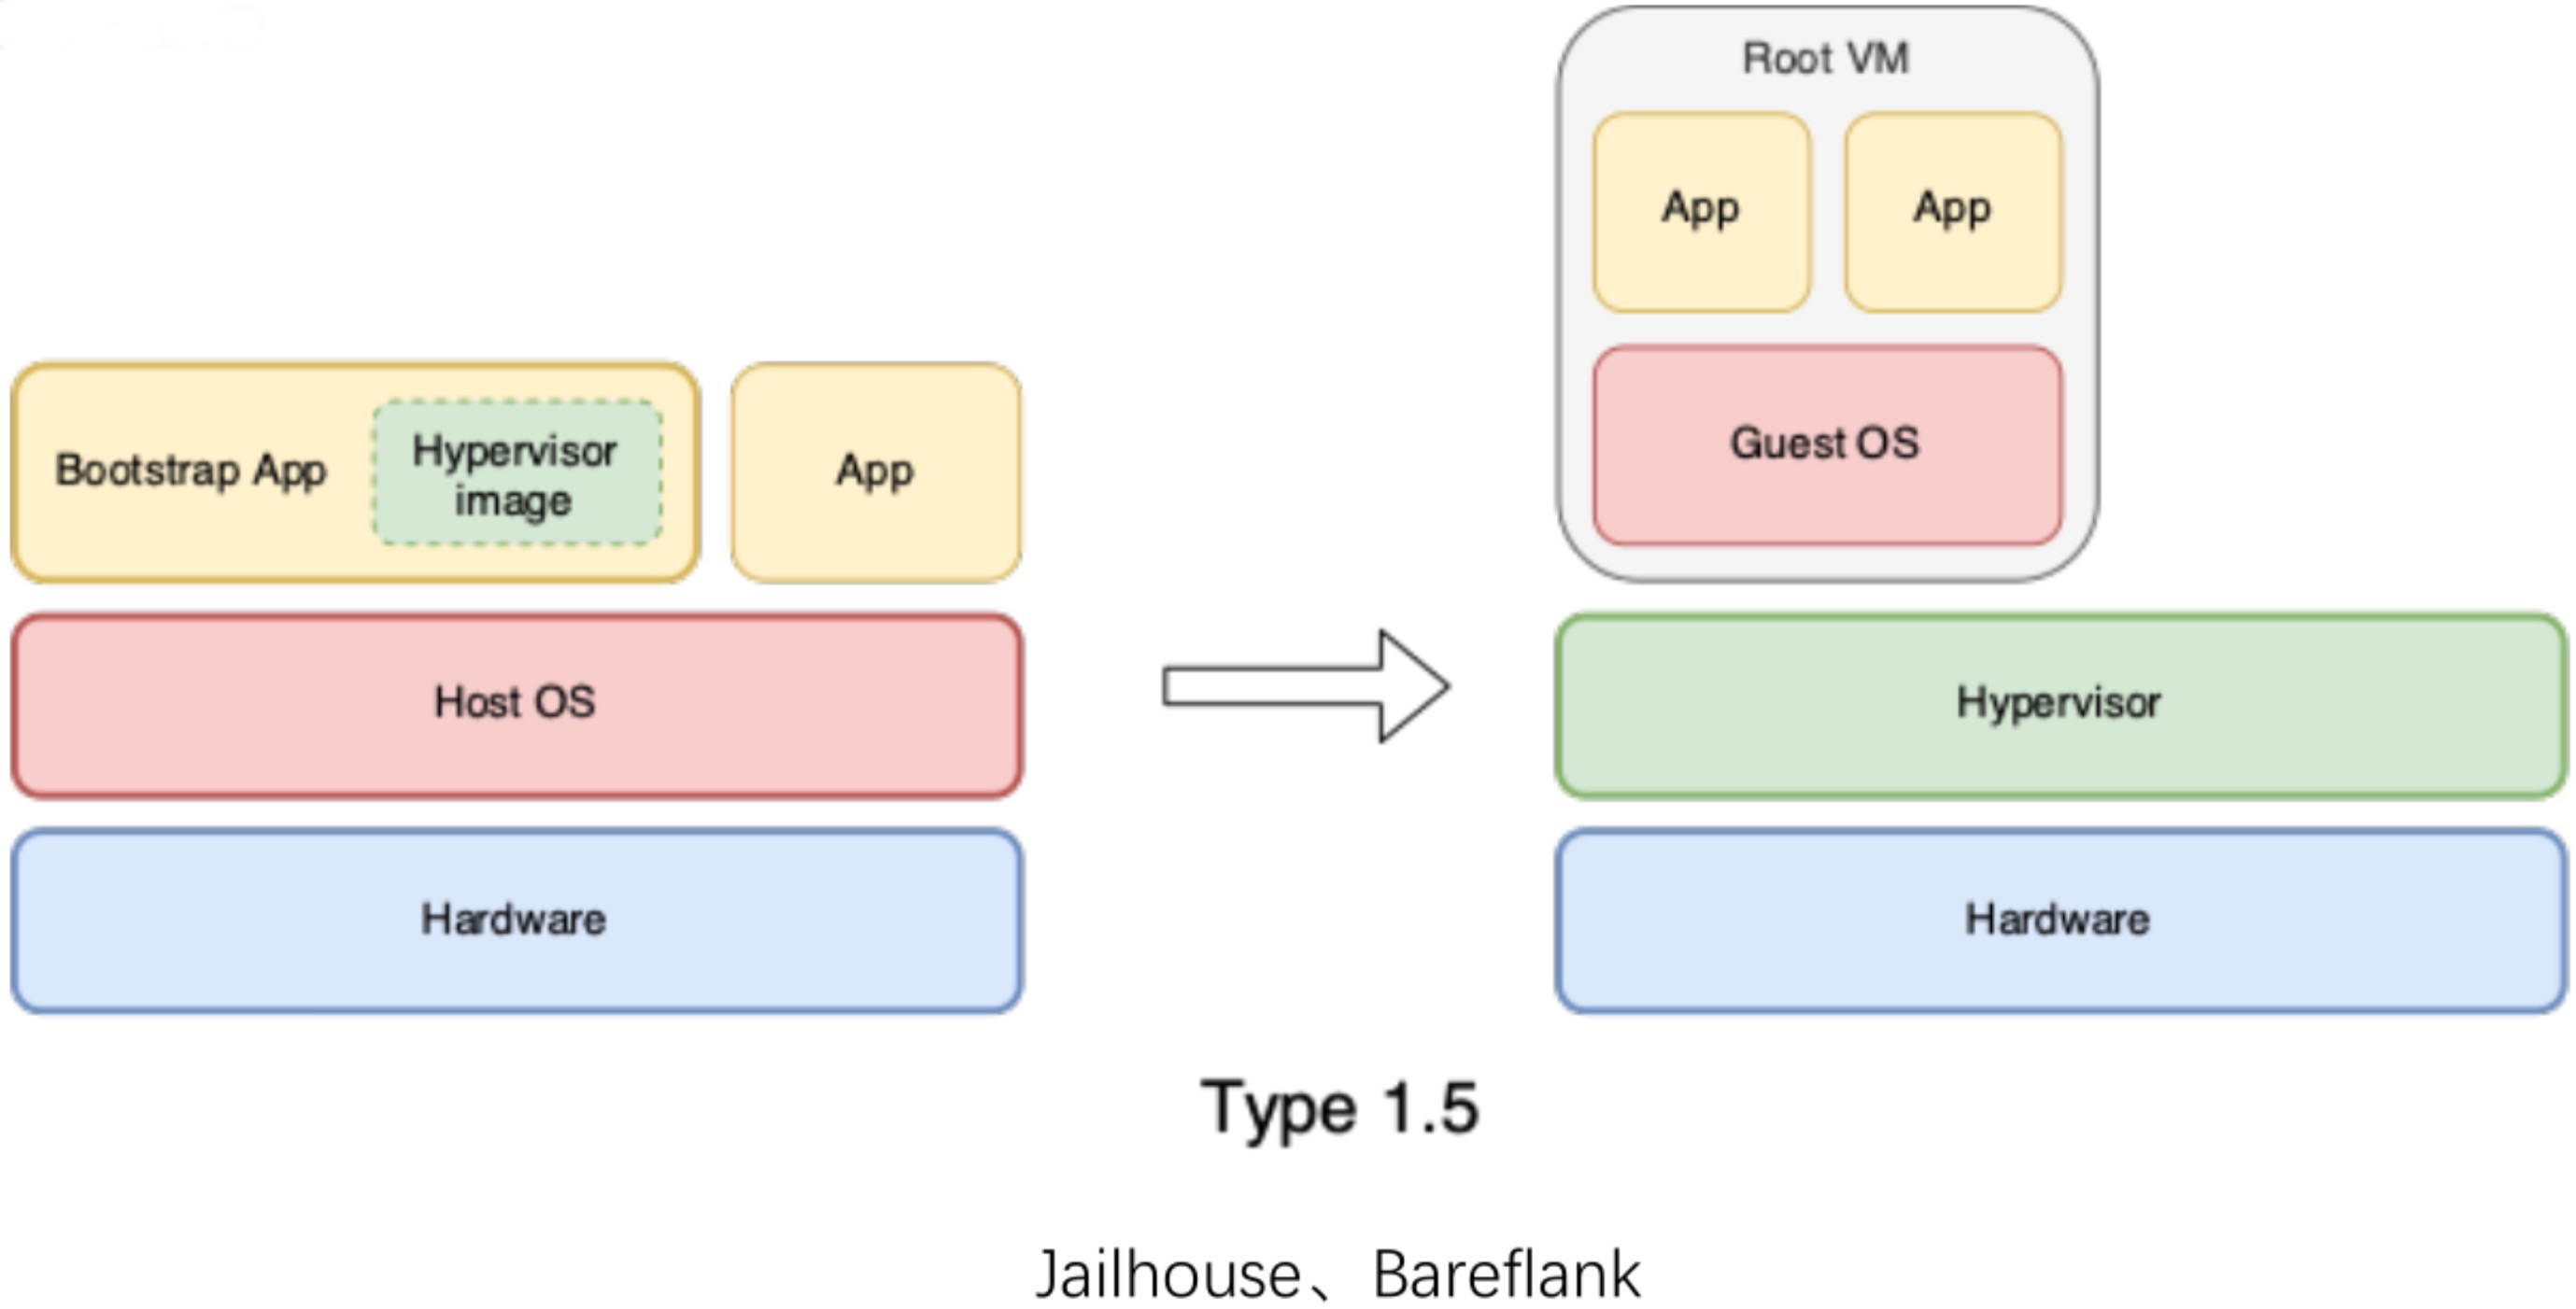
\includegraphics[width=0.9\textwidth]{figs/type-1.5-VMM.png}

\end{frame}
%----------------------------------------------
\begin{frame}
    \frametitle{RISC-V Hypervisor Extension}

            \centering
            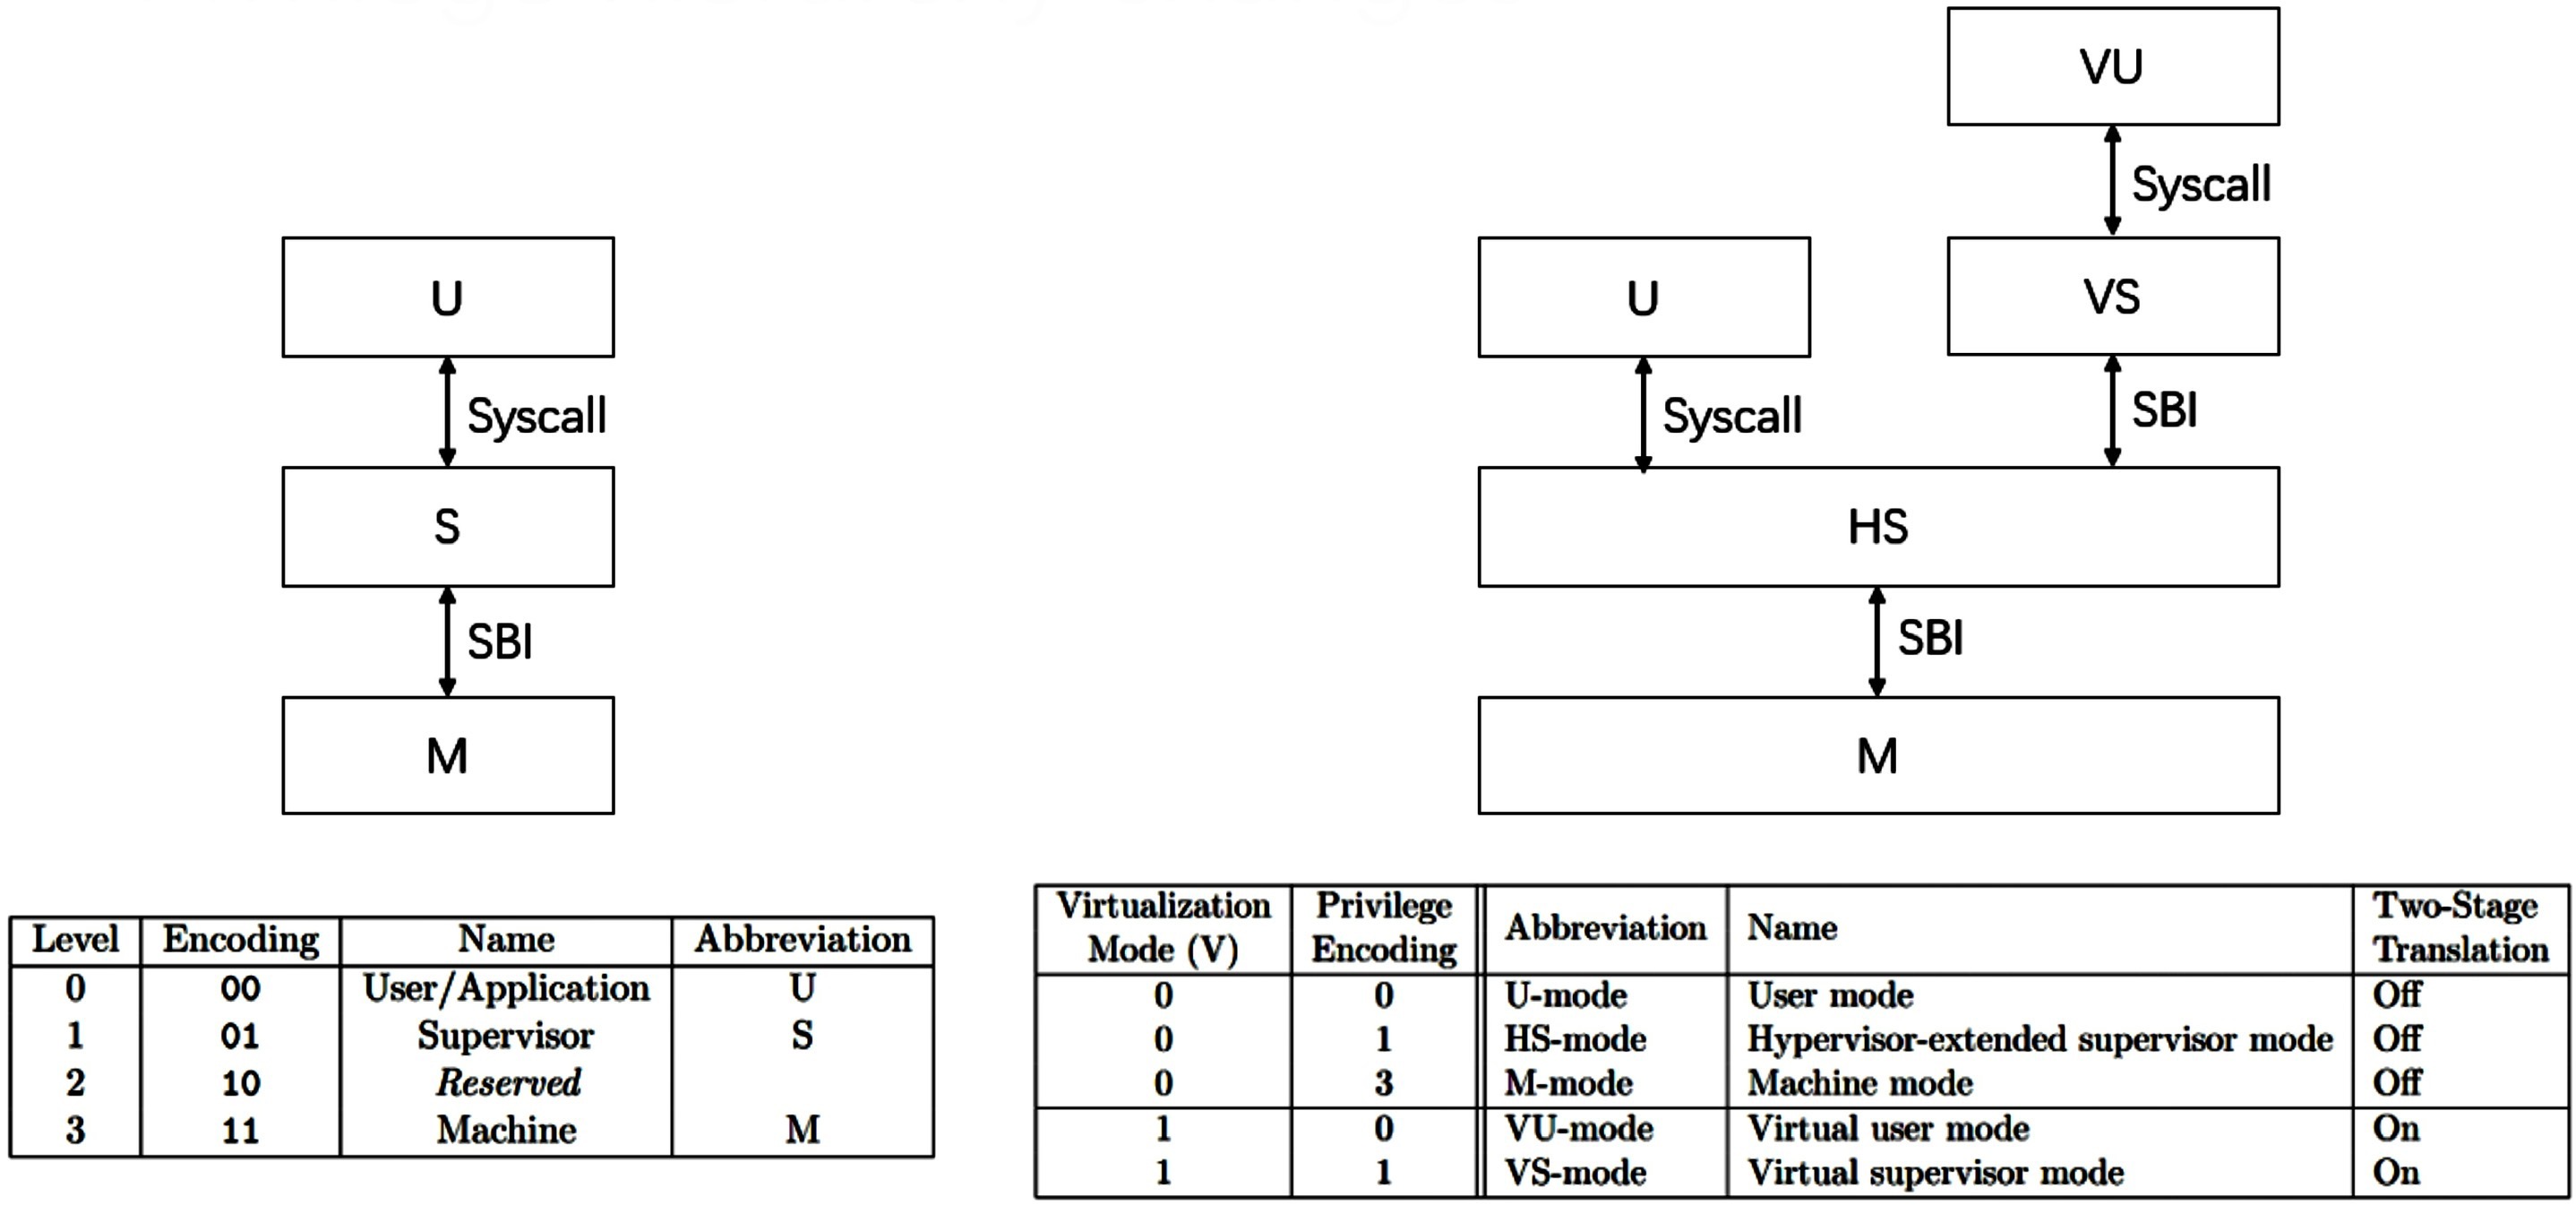
\includegraphics[width=1.0\textwidth]{figs/RV-Virtualization.png}

\end{frame}
%----------------------------------------------
\begin{frame}
\frametitle{提纲} % Table of contents slide, comment this block out to remove it
\tableofcontents % Throughout your presentation, if you choose to use \section{} and \subsection{} commands, these will automatically be printed on this slide as an overview of your presentation
\end{frame}
%-------------------------------------------------
\subsection{CPU Virtualization in VMM}
%-------------------------------------------------
\begin{frame}
	\frametitle{How VMM works }
	
	
	
	\begin{columns}
		
		\begin{column}{.3\textwidth}
			
			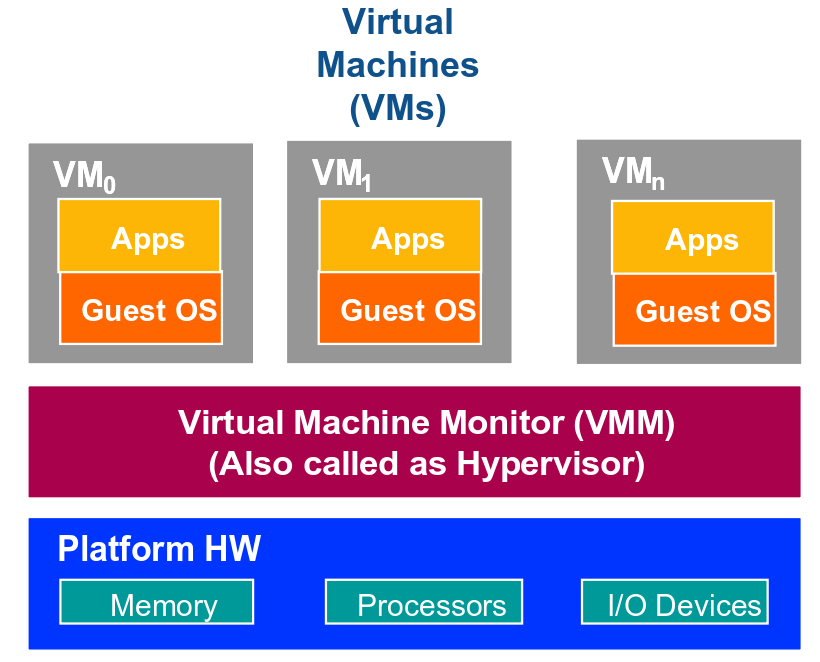
\includegraphics[width=1.\textwidth]{vmm-overview}
			
		\end{column}
		
		\begin{column}{.7\textwidth}
			
			Start with a “simpler” question:  how do (regular) machines work?	

			\centering
			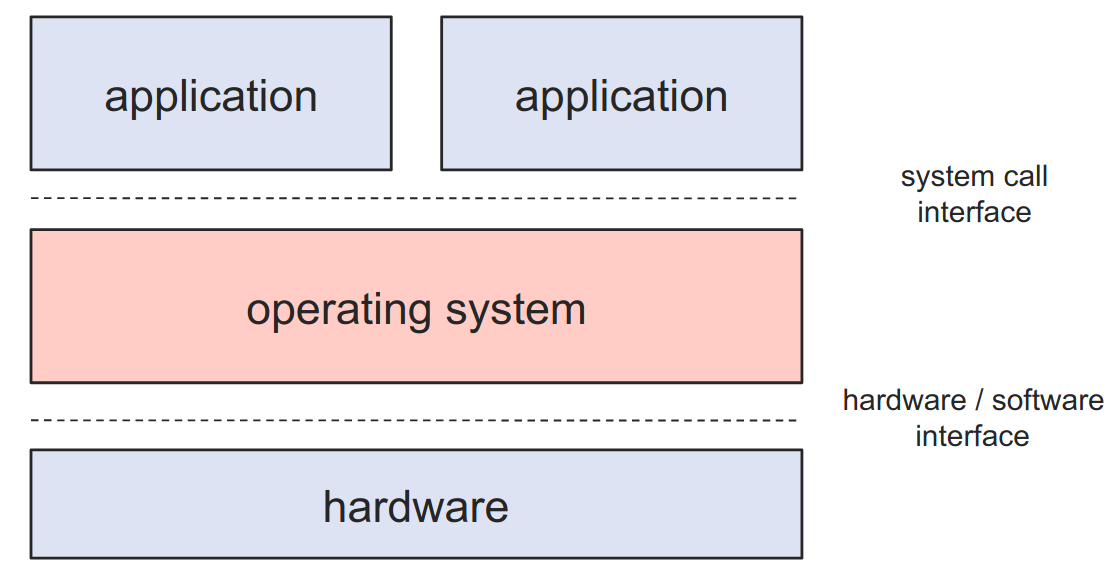
\includegraphics[width=.7\textwidth]{os-do-work}	
			
			\begin{itemize}
				\item What is computer hardware? (CPU, MEM, IO)
				\item What is an OS? 
				\item What is an application? (relies on the system call interface)
				
			\end{itemize} 
				
		\end{column}
		
		
	\end{columns}
	
	
\end{frame}


%-------------------------------------------------
\begin{frame}
	\frametitle{Executing a System Call}
	
	
	
	\begin{columns}
		
		\begin{column}{.3\textwidth}
			
			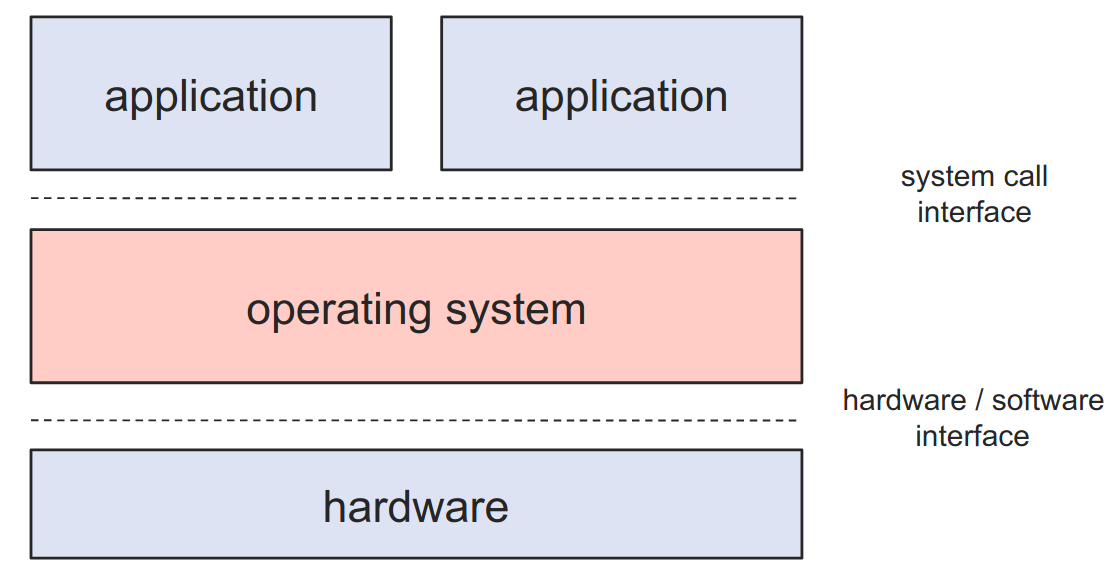
\includegraphics[width=1.\textwidth]{os-do-work}
			
		\end{column}
		
		\begin{column}{.7\textwidth}
			
			Start with a “simpler” question:  how do (regular) machines work?	
			
			\centering
			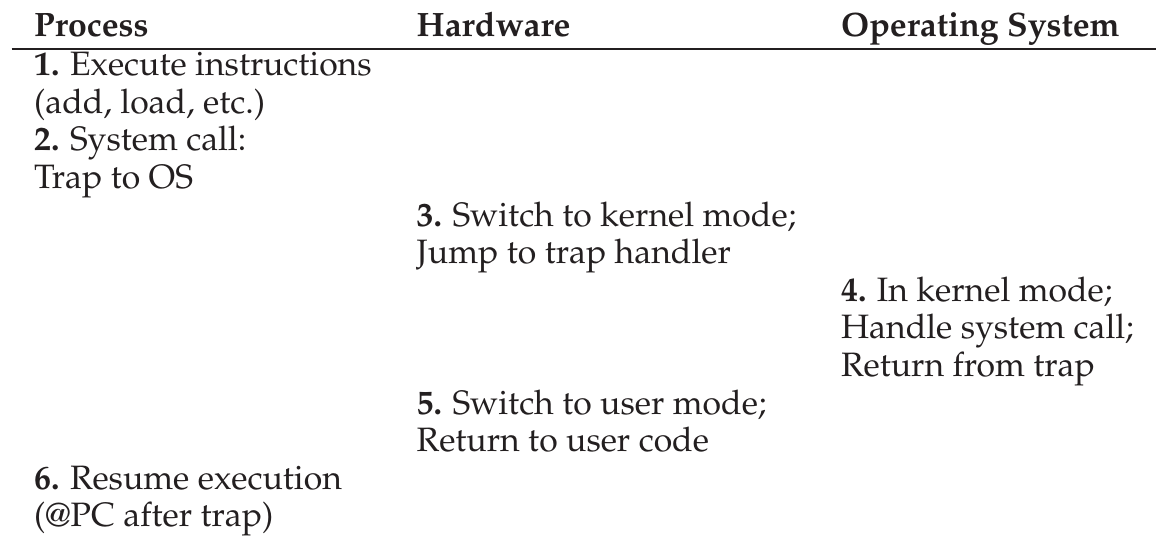
\includegraphics[width=1.\textwidth]{exec-syscall}	
			
			% Executing a System Call
			
%			\begin{itemize}
%				\item What is computer hardware? (CPU, MEM, IO)
%				\item What is an OS? 
%				\item What’s an application? (relies on the system call interface)
%				
%			\end{itemize} 
			
		\end{column}
		
		
	\end{columns}
	
	
\end{frame}

%-------------------------------------------------
\begin{frame}
	\frametitle{Run kernel as a user-level program}
	
	
	
	\begin{columns}
		
		\begin{column}{.3\textwidth}
			
			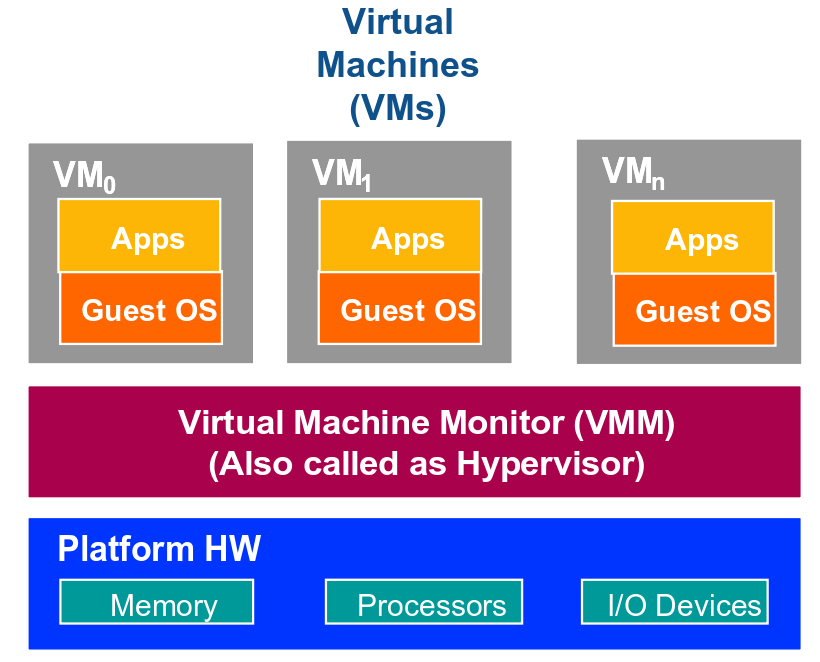
\includegraphics[width=1.0\textwidth]{vmm-overview}
			
		\end{column}
		
		\begin{column}{.7\textwidth}
			
			What if we run the Linux/Windows kernel as a user-level program?	
			
			\centering
			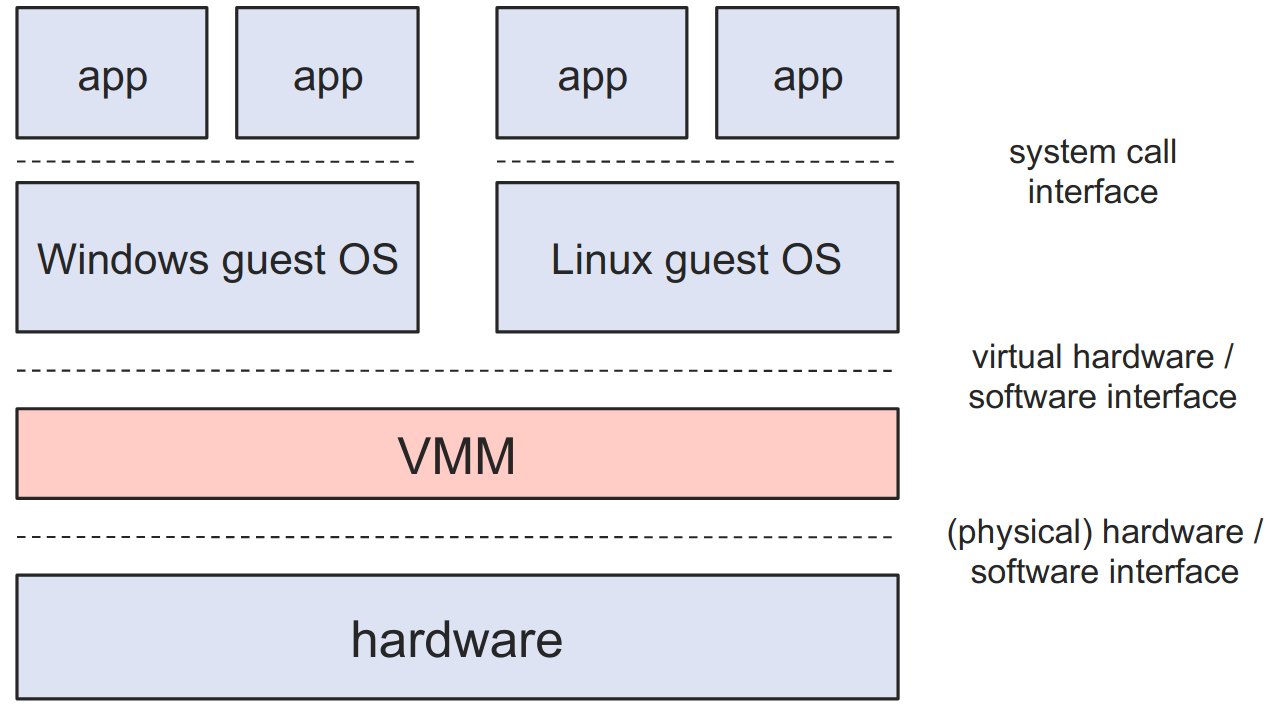
\includegraphics[width=.65\textwidth]{vmm-do-work}	
			
			\begin{itemize}
				\item What happens when Linux issues a sensitive instruction?
				\item What (virtual) hardware devices should Windows see?  
				\item How do you prevent apps running on Linux from hurting Linux?
				
			\end{itemize} 
			
		\end{column}
		
		
	\end{columns}
	
	
\end{frame}


%-------------------------------------------------
\begin{frame}
	\frametitle{System Call with Virtualization}
	
	
	
	\begin{columns}
		
		\begin{column}{.3\textwidth}
			
			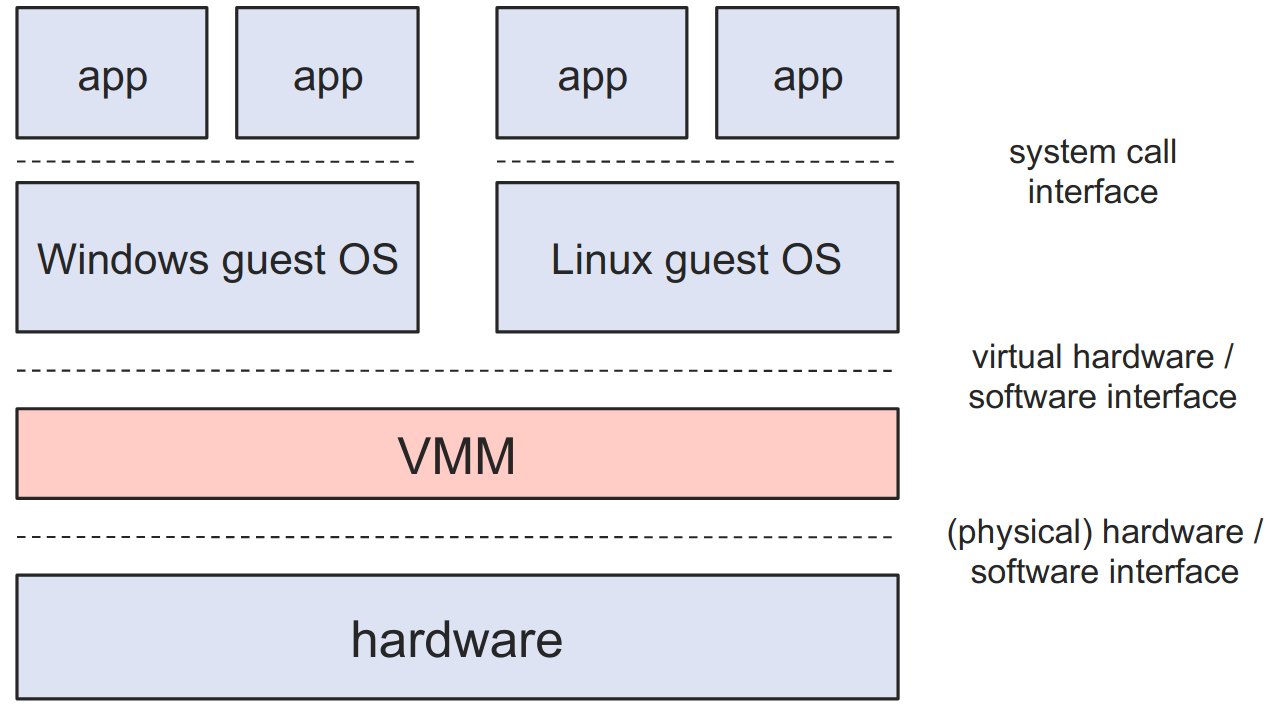
\includegraphics[width=1.\textwidth]{vmm-do-work}
			
		\end{column}
		
		\begin{column}{.7\textwidth}
			
			What if we run the Linux/Windows kernel as a user-level program?	
			
			\centering
			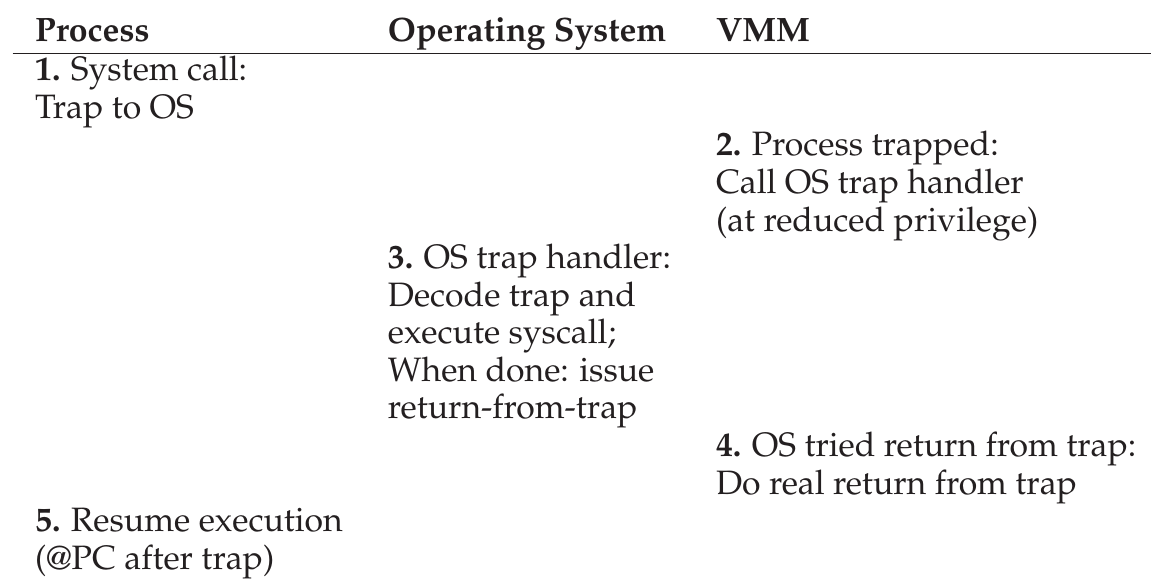
\includegraphics[width=1.\textwidth]{exec-syscall-in-vmm}	
			
			System Call Flow with Virtualization
			
			
		\end{column}
		
		
	\end{columns}
	
	
\end{frame}

%-------------------------------------------------
\begin{frame}
	\frametitle{Privileged Instruction and Sensitive Instruction}

	\begin{columns}
		
		\begin{column}{.35\textwidth}
			
			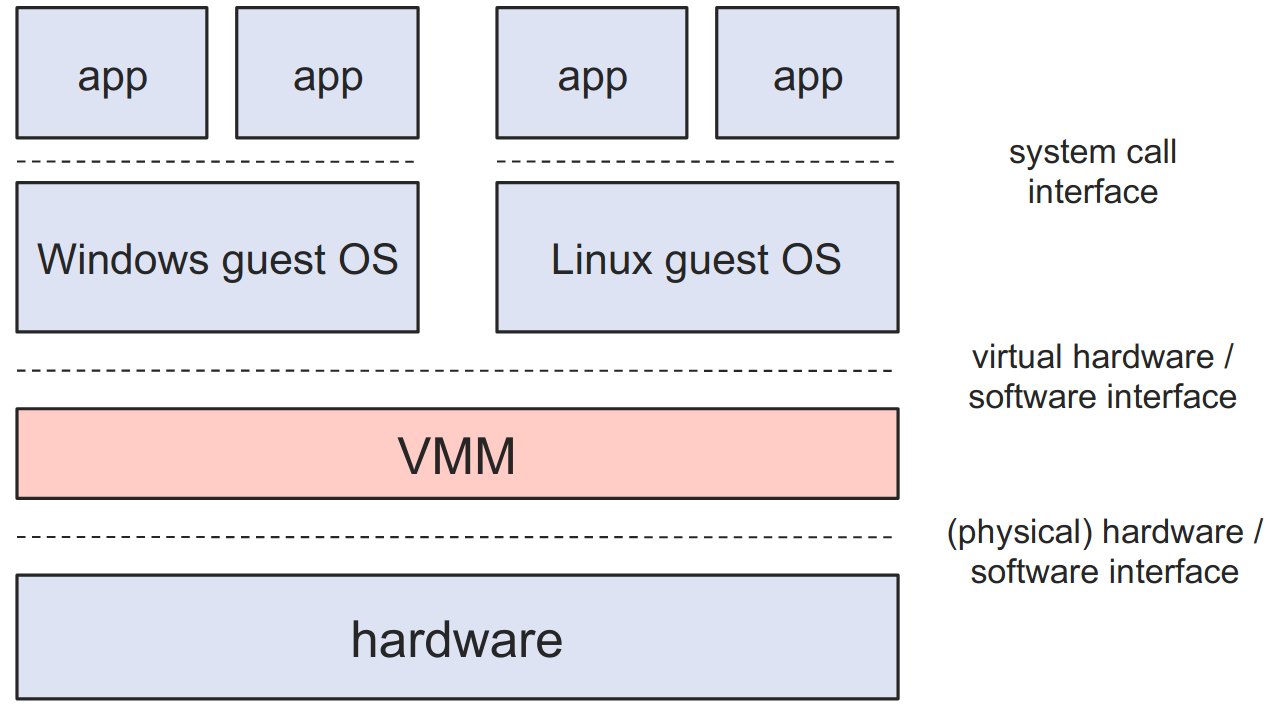
\includegraphics[width=.9\textwidth]{vmm-do-work}	
			
		\end{column}
		
		\begin{column}{.65\textwidth}
			
			What if we run the Linux/Windows kernel as a user-level program?	
		\begin{itemize}
			\item Rely on CPU to trap sensitive instructions and hand off to VMM
			\begin{itemize}
				\item VMM emulates the effect of sensitive instruction on the virtual hardware that it provides to its guest OSs 
				\item VMM provides a virtual HW/SW interface to guest OSs by trapping and emulating sensitive instructions 
				
			\end{itemize} 
		\end{itemize} 
		\end{column}
		
		
	\end{columns}
	
	
\end{frame}



%-------------------------------------------------
\begin{frame}
	\frametitle{Privileged Instruction and Sensitive Instruction}
	
	\begin{columns}
		
		\begin{column}{.35\textwidth}
			
			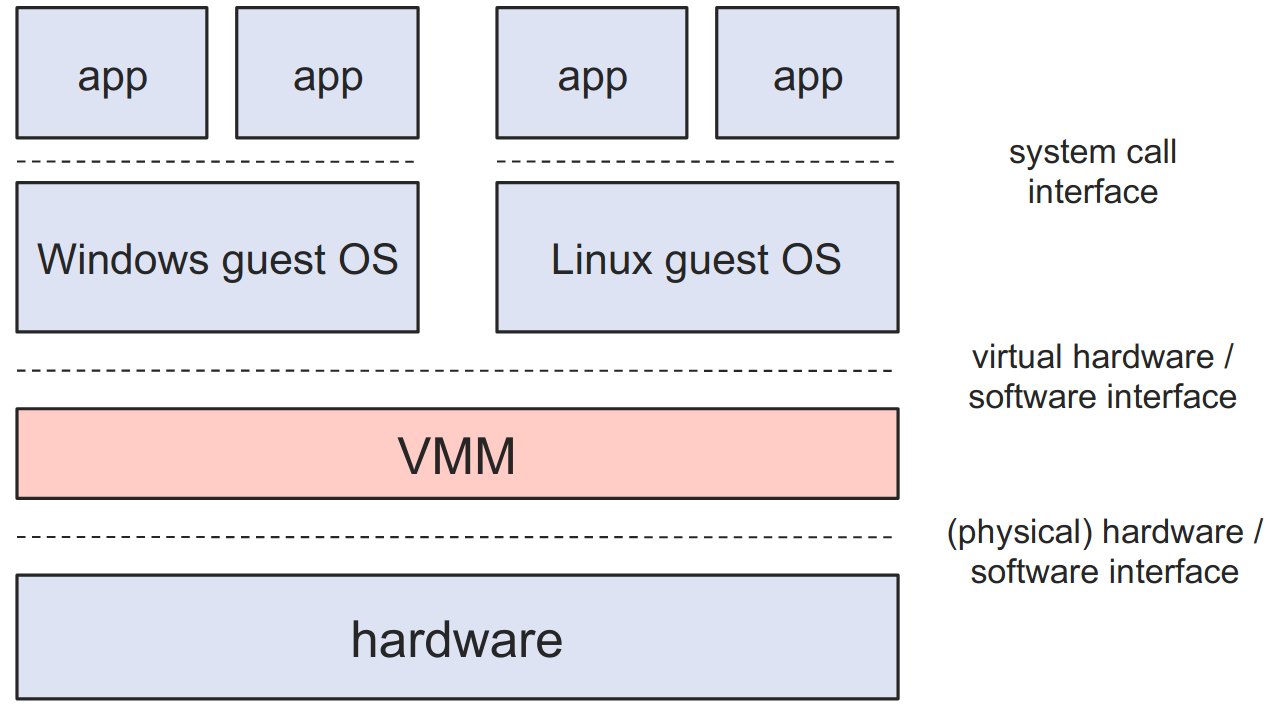
\includegraphics[width=.9\textwidth]{vmm-do-work}	
			
		\end{column}
		
		\begin{column}{.65\textwidth}
			What if we run the Linux/Windows kernel as a user-level program?	
			
			\begin{flushleft}
				Goldberg (1974):  two classes of instructions 
			\end{flushleft}
			\begin{itemize}
				\item privileged instructions:   those that trap when CPU is in user-mode  
				\item sensitive instructions:   those that modify hardware configuration or resources, and those whose behavior depends on HW configuration 
				
			\end{itemize} 
			
		\end{column}
		
		
	\end{columns}
	
	
\end{frame}

%-------------------------------------------------
\begin{frame}
	\frametitle{CPU Virtualization in VMM}
	
	\begin{columns}
		
		\begin{column}{.35\textwidth}
			
			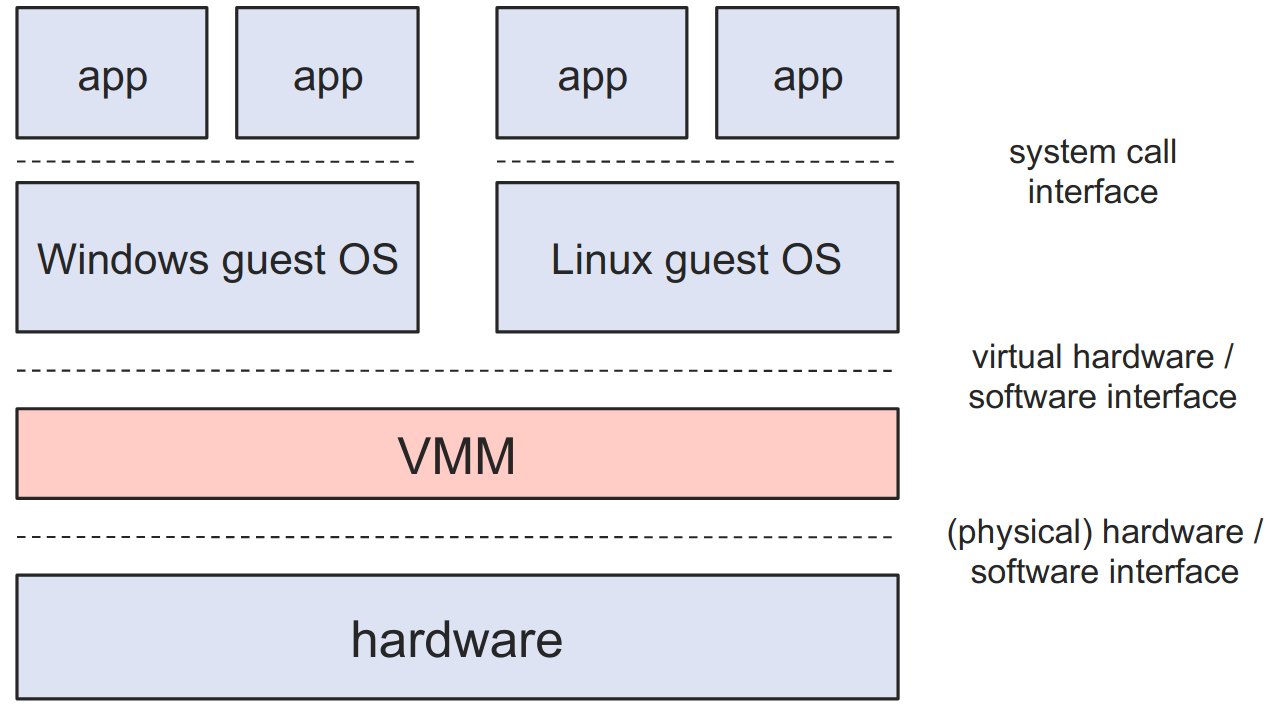
\includegraphics[width=.9\textwidth]{vmm-do-work}	
			
		\end{column}
		
		\begin{column}{.65\textwidth}
			What if we run the Linux/Windows kernel as a user-level program?	
			
			\begin{flushleft}
				\textbf{A VMM can be constructed efficiently and safely if the set of sensitive instructions is a subset of the set of privileged instructions.}
			\end{flushleft}
%			\begin{itemize}
%				\item privileged instructions:   those that trap when CPU is in user-mode  
%				\item sensitive instructions:   those that modify hardware configuration or resources, and those whose behavior depends on HW configuration 
%				
%			\end{itemize} 
		\end{column}
	\end{columns}
\end{frame}
%-------------------------------------------------
\begin{frame}
    \frametitle{Intel VT-x指令扩展}
    \begin{columns}
        
        \begin{column}{.6\textwidth}
            
            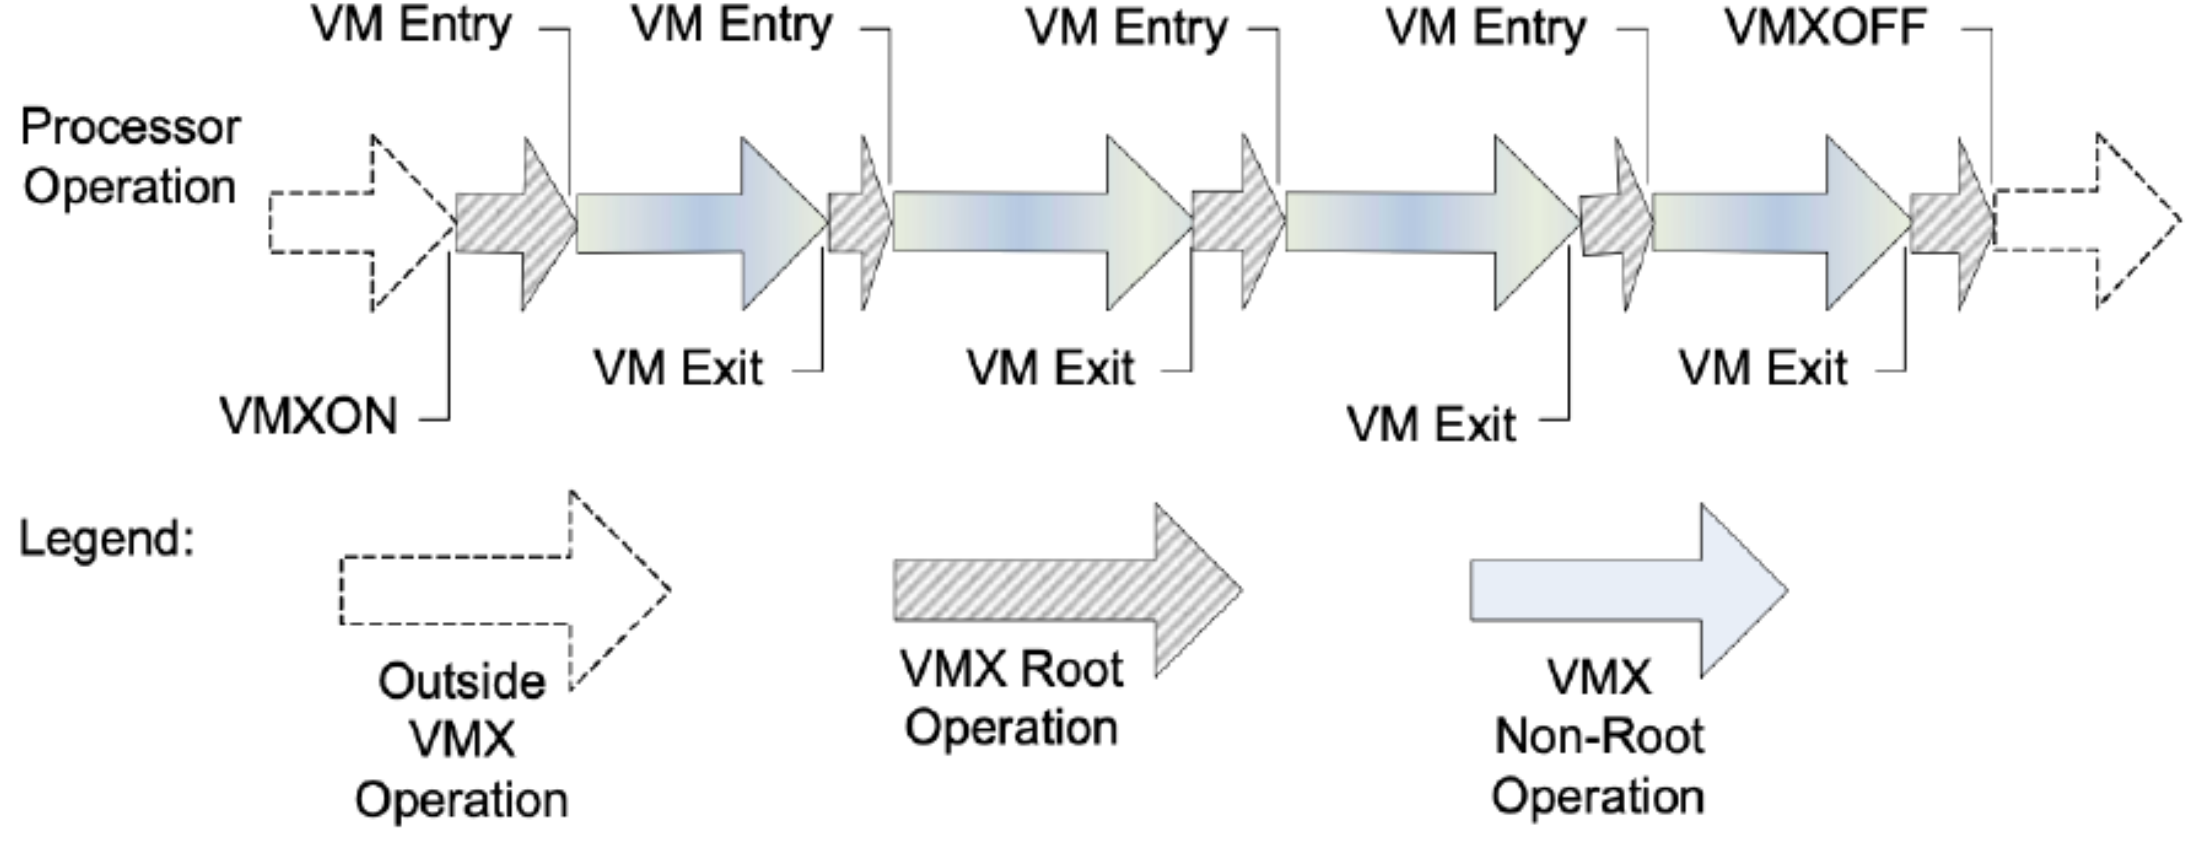
\includegraphics[width=1.\textwidth]{figs/Intel-VT-x.png}
            
        \end{column}
        
        \begin{column}{.4\textwidth}
            \begin{itemize}
                \item Virtual-Machine eXtensions (VMX)
                \item 开启VMX后的特殊模式
                \begin{itemize}
                    \item VMX root operation
                    \item VMX non-root operation
                \end{itemize} 
                \item VM Entry/VM Exit
            \end{itemize} 
        \end{column}
    \end{columns}
\end{frame}
%----------------------------------------------
\begin{frame}
\frametitle{提纲} % Table of contents slide, comment this block out to remove it
\tableofcontents % Throughout your presentation, if you choose to use \section{} and \subsection{} commands, these will automatically be printed on this slide as an overview of your presentation
\end{frame}
%-------------------------------------------------
\subsection{VMM Memory Virtualization}
%-------------------------------------------------
\begin{frame}
	\frametitle{Address Translation in VMM}
	
	
	
	\begin{columns}
		
		\begin{column}{.25\textwidth}
			
			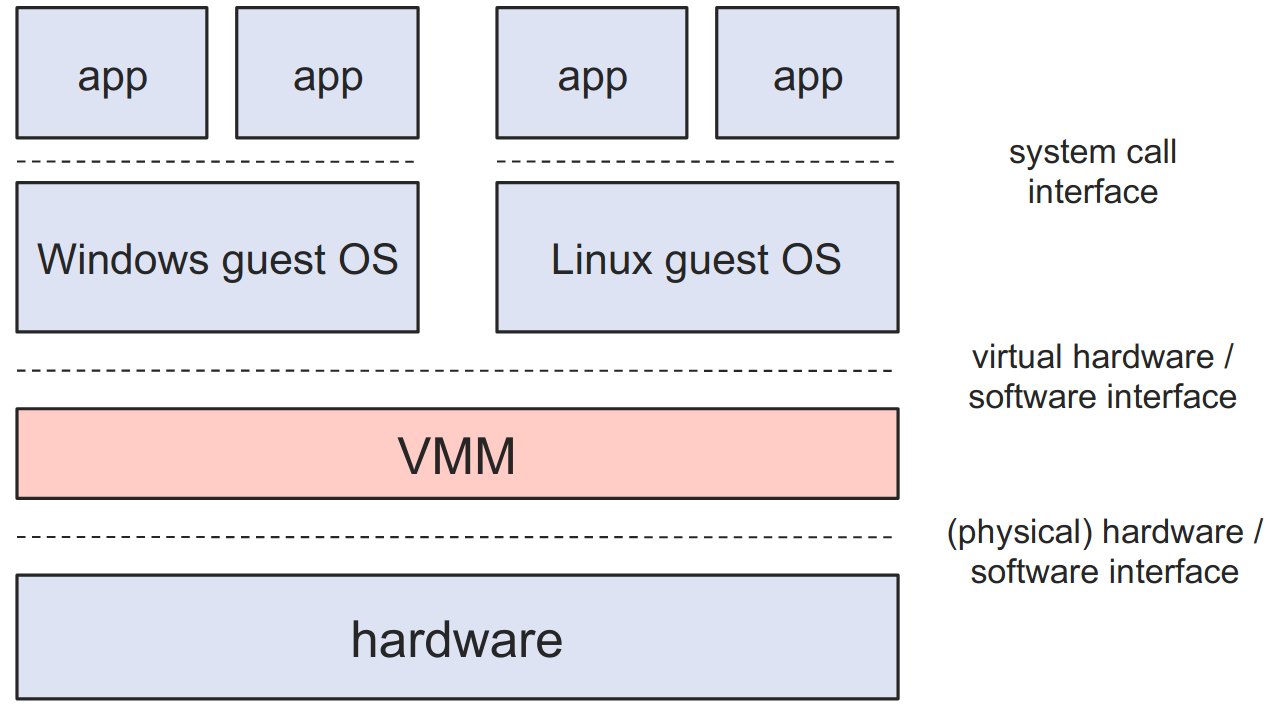
\includegraphics[width=1.\textwidth]{vmm-do-work}
			
		\end{column}
		
		\begin{column}{.75\textwidth}
			
%			What if we run the Linux/Windows kernel as a user-level program?	
			
			\centering
			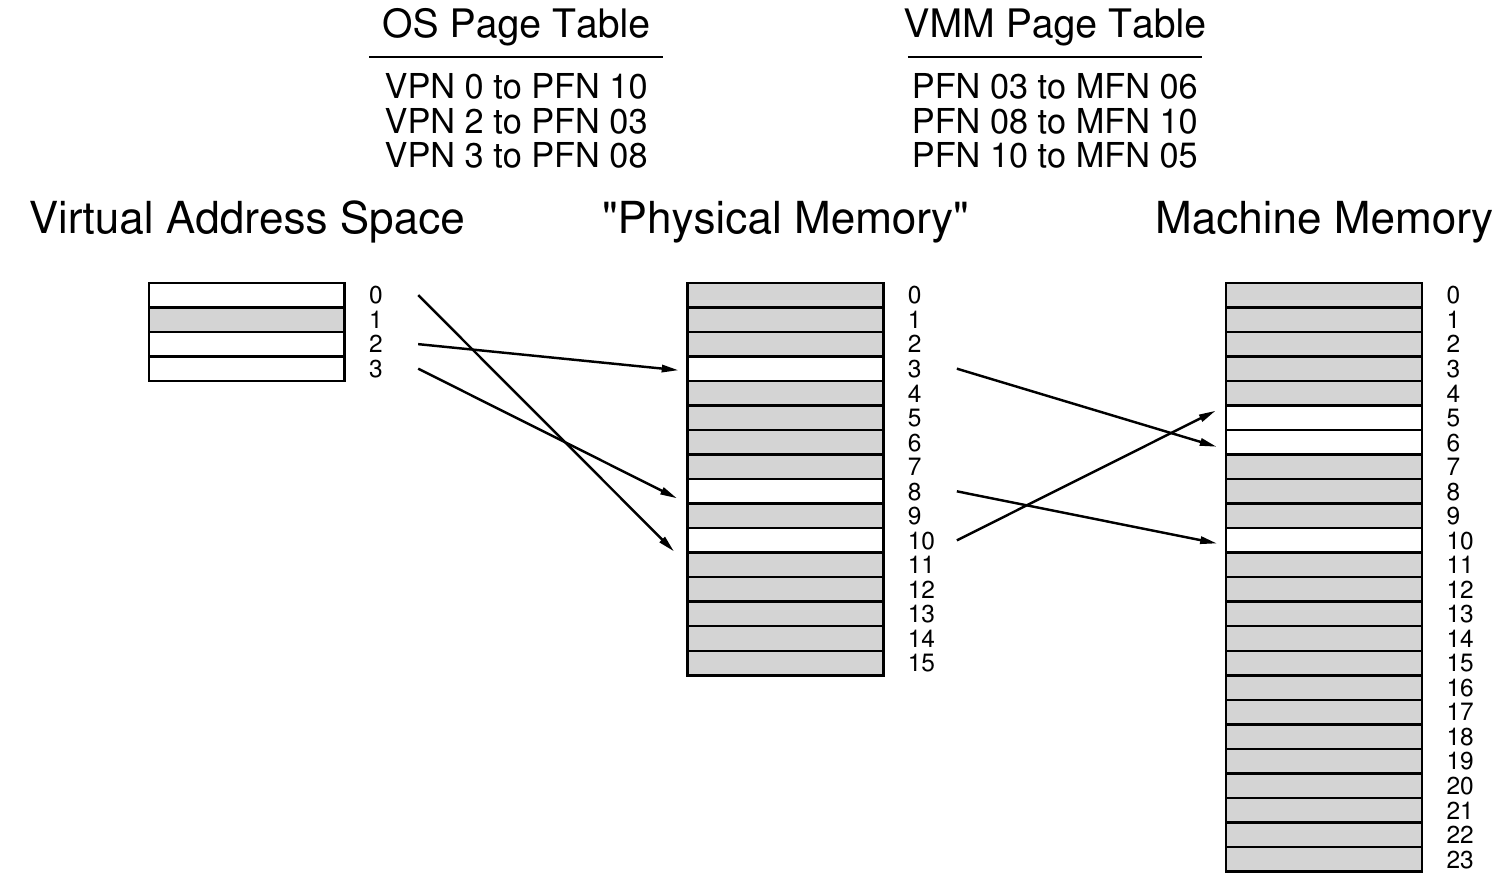
\includegraphics[width=1.\textwidth]{vmm-address-space}	

		\end{column}
		
		
	\end{columns}
	
	
\end{frame}


%-------------------------------------------------
\begin{frame}
	\frametitle{TLB Miss without Virtualization}
	
	
	
	\begin{columns}
		
		\begin{column}{.25\textwidth}
			
			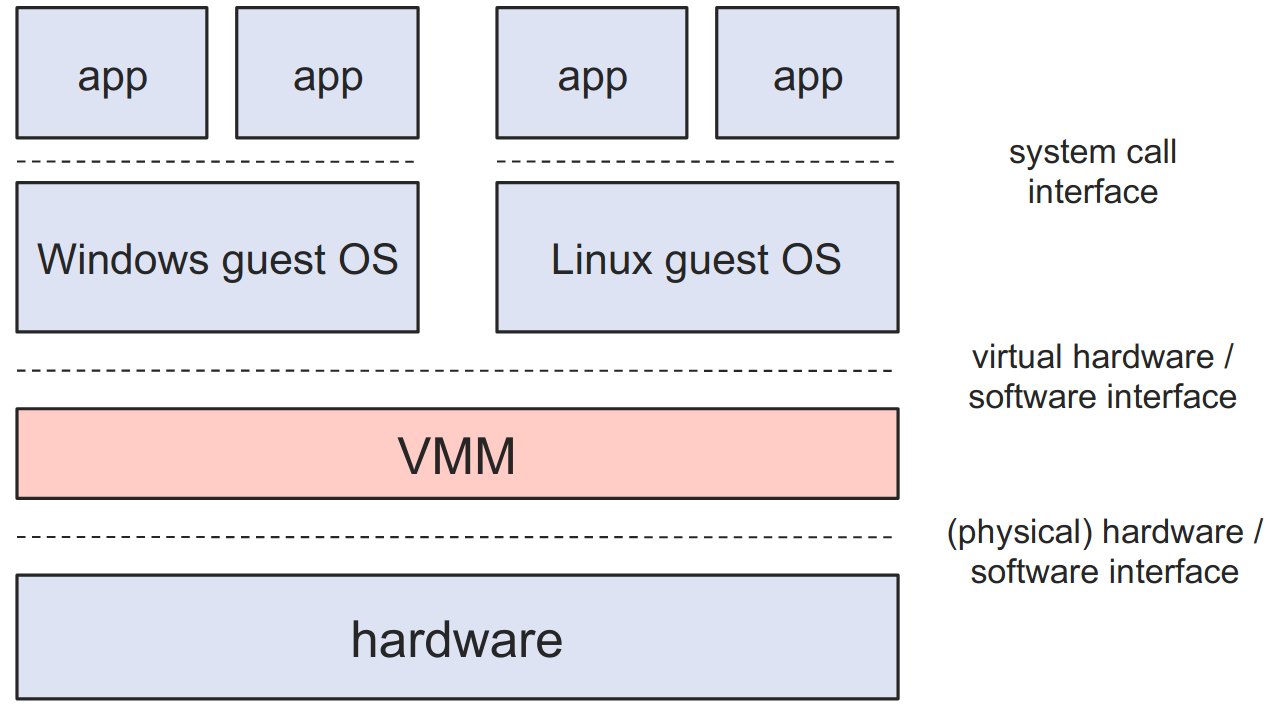
\includegraphics[width=1.\textwidth]{vmm-do-work}
			
		\end{column}
		
		\begin{column}{.75\textwidth}
			
			%			What if we run the Linux/Windows kernel as a user-level program?	
			
			\centering
			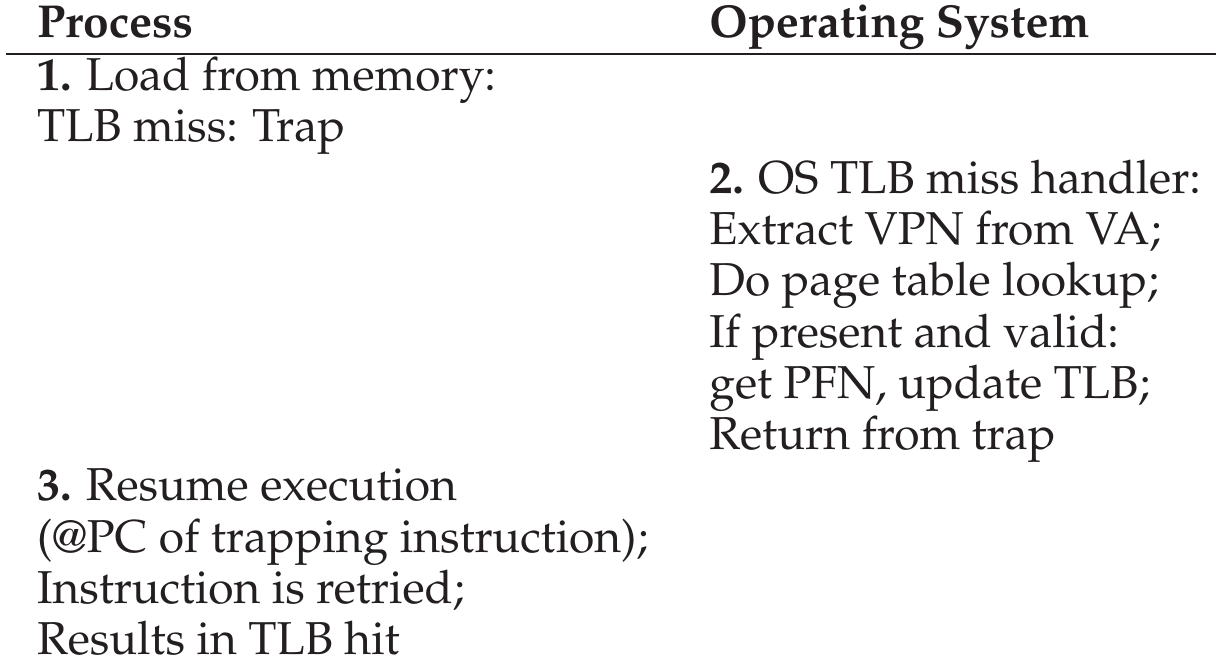
\includegraphics[width=.9\textwidth]{os-tlbmiss}	
			%			\begin{flushleft}
			
			\textbf{TLB Miss Flow without Virtualization}
			
			%			\end{flushleft}
			
			
		\end{column}
		
		
	\end{columns}
	
	
\end{frame}


%-------------------------------------------------
\begin{frame}
	\frametitle{TLB Miss Flow with Virtualization}
	
	
	
	\begin{columns}
		
		\begin{column}{.2\textwidth}
			\centering
			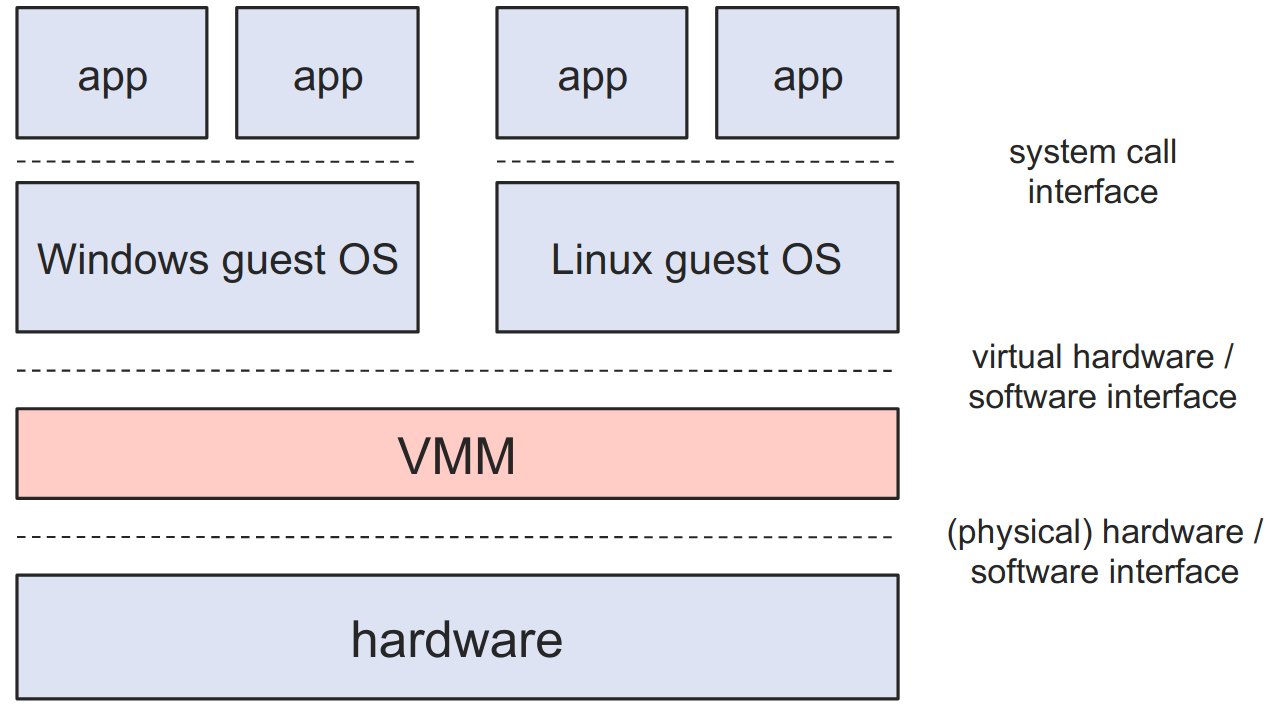
\includegraphics[width=1.\textwidth]{vmm-do-work}
			
		\end{column}
		
		\begin{column}{.8\textwidth}
			
			%			What if we run the Linux/Windows kernel as a user-level program?	
			
			\centering
			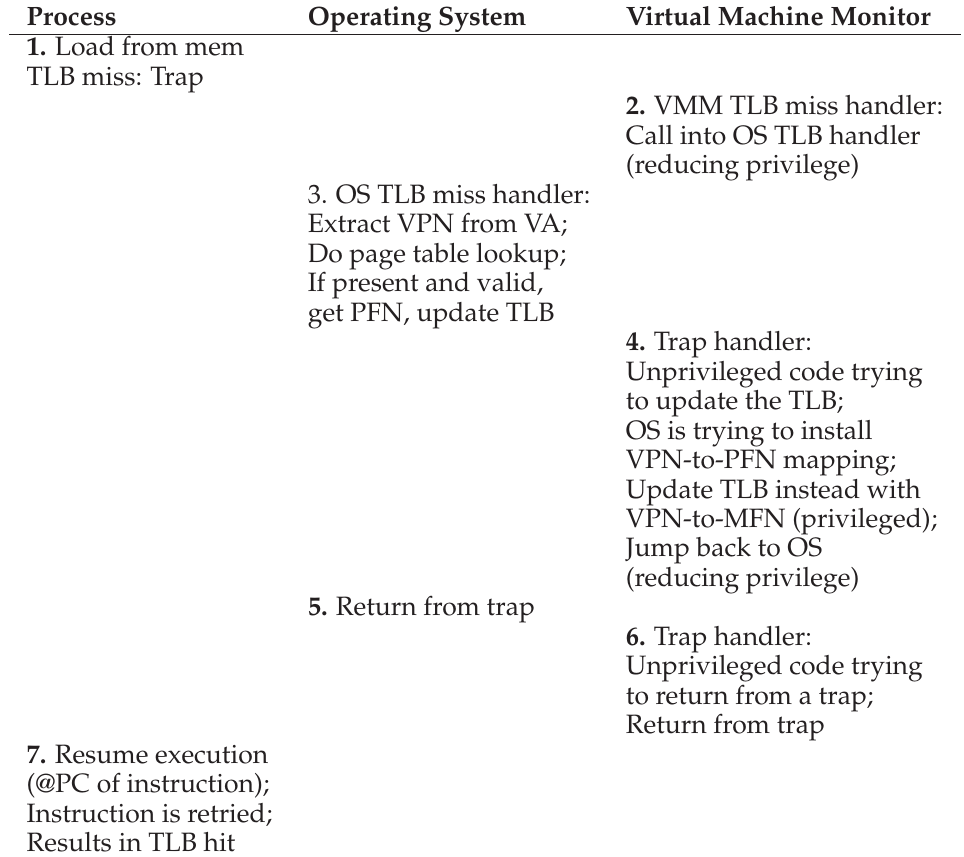
\includegraphics[width=.65\textwidth]{vmm-tlbmiss}	
			%			\begin{flushleft}
			
			%TLB Miss Flow with Virtualization
			
			%			\end{flushleft}
			
			
		\end{column}
		
		
	\end{columns}
	
	
\end{frame}

%-------------------------------------------------
\begin{frame}
	\frametitle{hardware-managed TLB}
	
	
	
	\begin{columns}
		
		\begin{column}{.4\textwidth}
			\centering
			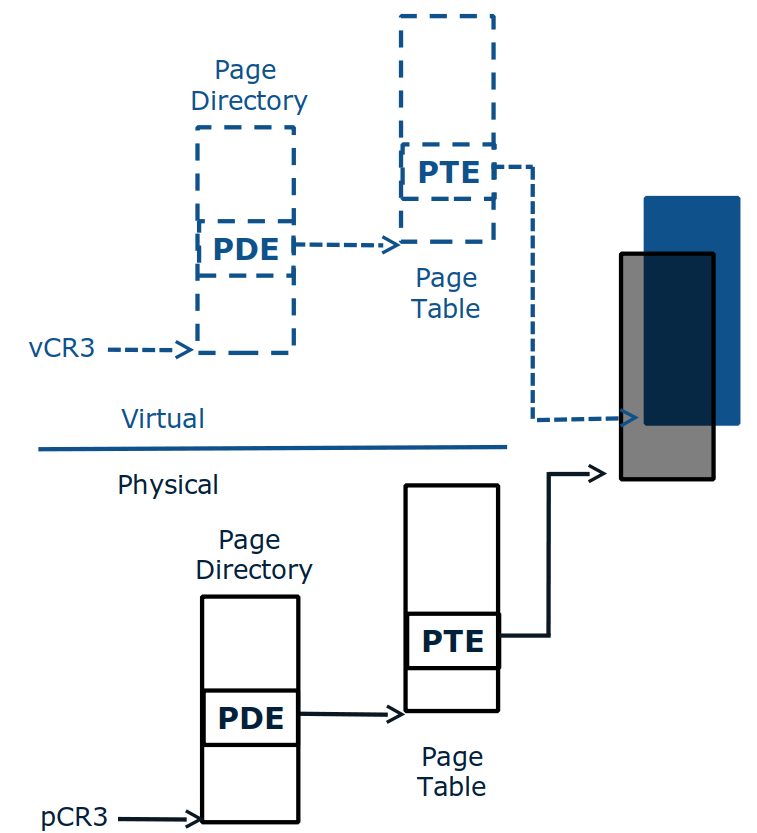
\includegraphics[width=1.\textwidth]{shadow-page-table}
			
		\end{column}
		
		\begin{column}{.6\textwidth}
			
			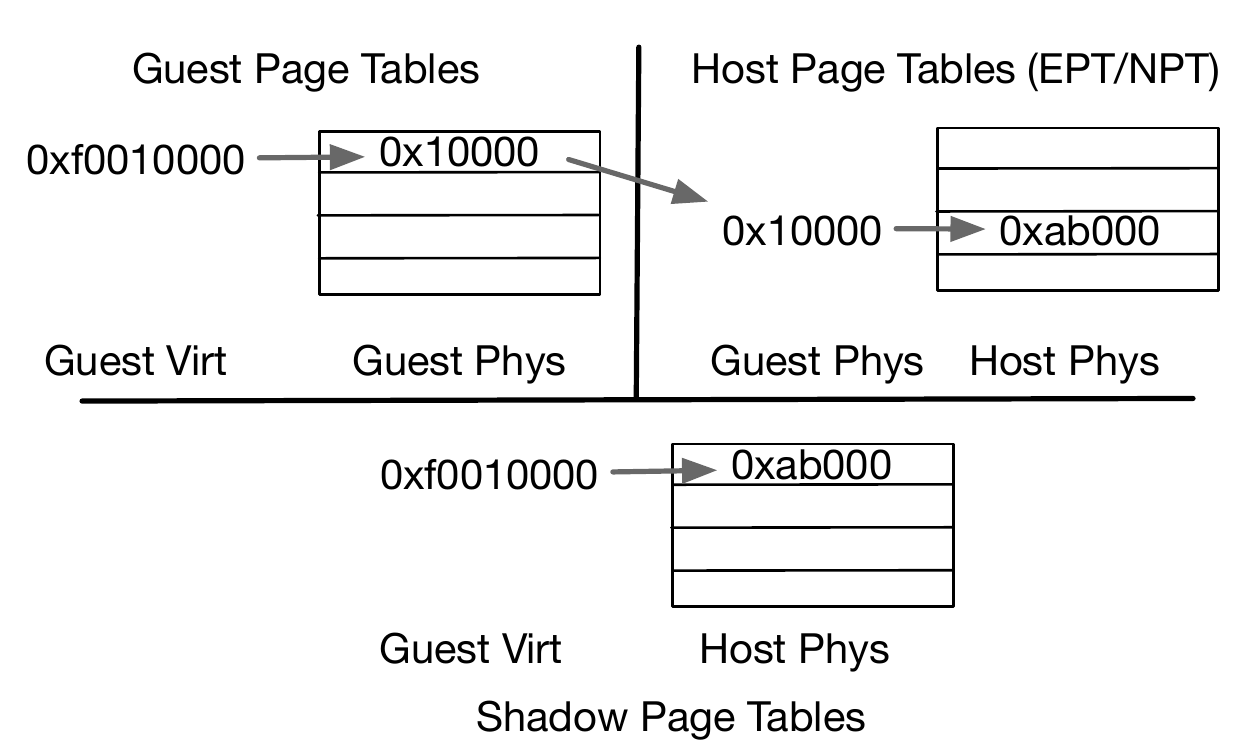
\includegraphics[width=1.\textwidth]{gpt-ept-spt}
			 How does the virtual machine monitor get involved with a
			hardware-managed TLB?	
			
%			\begin{itemize}
%				\item VMM doesn't have a chance to run on each TLB miss to sneak its translation into the system. 
%				\item VMM must closely monitor changes	the OS makes to each page table
%				\item VMM must keep a \textbf{shadow page table} that maps the virtual addresses of each process to the VMM's desired machine pages
%				\item VMM installs a process's \textbf{shadow page table }whenever the OS tries to install the process's	OS-level page table
%				
%			\end{itemize} 

			
			
		\end{column}
		
		
	\end{columns}
	
	
\end{frame}


%-------------------------------------------------
\begin{frame}
	\frametitle{Shadow Page Table}
	
	
	
	\begin{columns}
		
		\begin{column}{.4\textwidth}
			\centering
			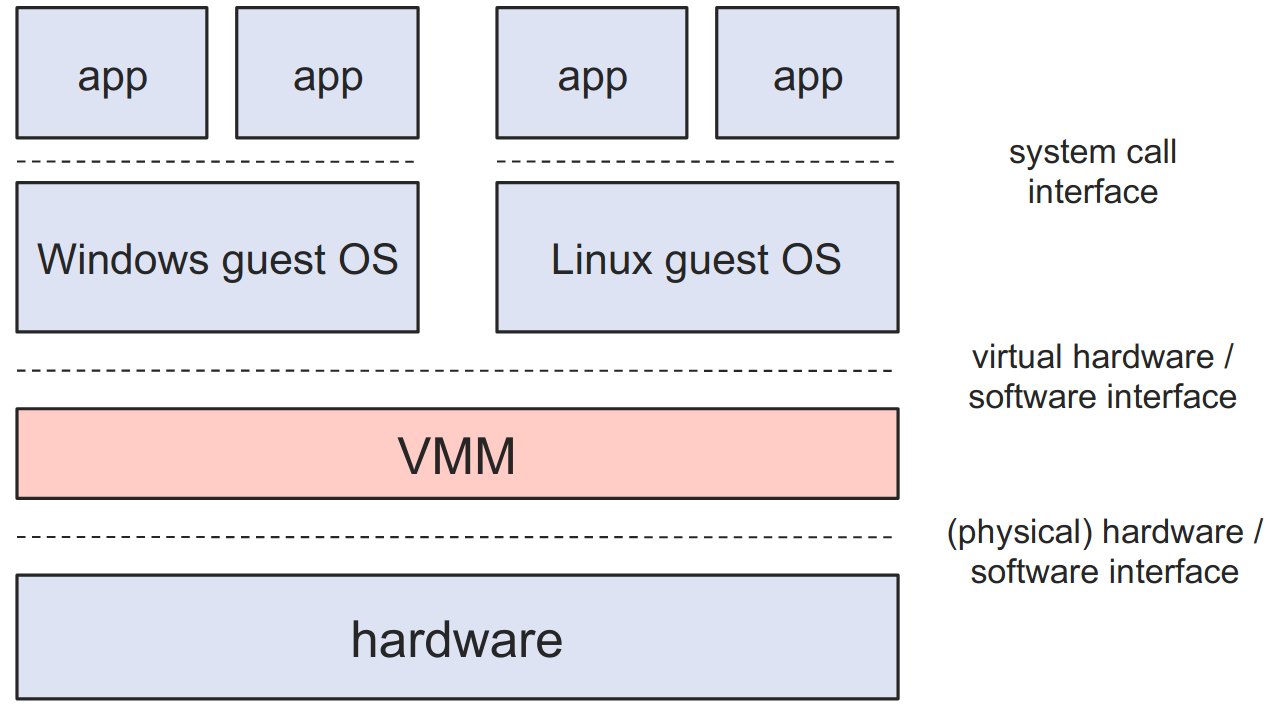
\includegraphics[width=.6\textwidth]{vmm-do-work}
			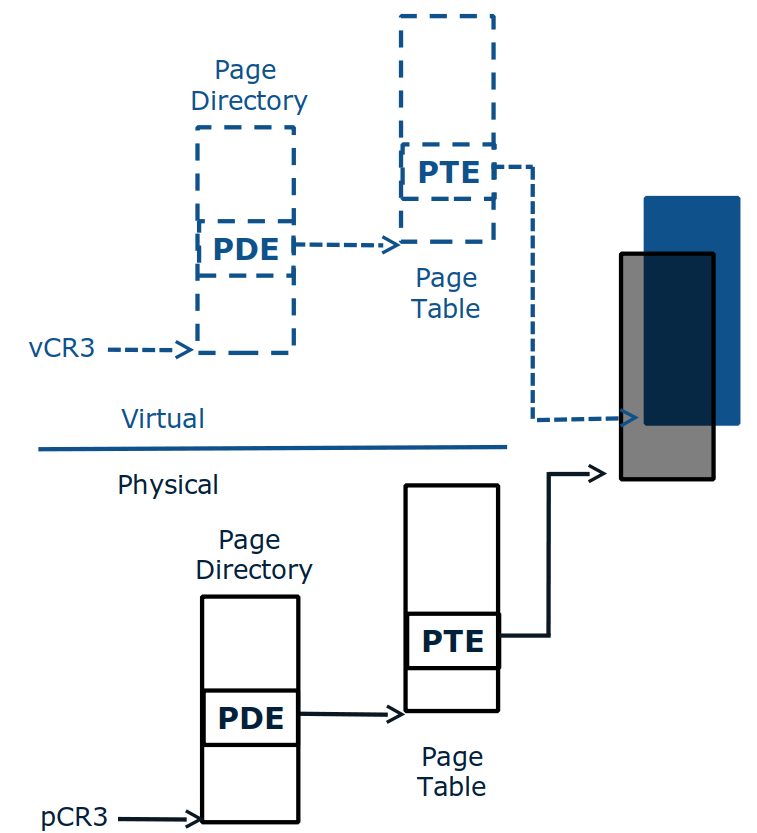
\includegraphics[width=.6\textwidth]{shadow-page-table}
		\end{column}
		
		\begin{column}{.6\textwidth}
			
			How does the virtual machine monitor get involved with a
			hardware-managed TLB?	
			
			\begin{itemize}
				\item VMM doesn't have a chance to run on each TLB miss to sneak its translation into the system. 
				\item VMM must closely monitor changes	the OS makes to each page table
				\item VMM must keep a \textbf{shadow page table} that maps the virtual addresses of each process to the VMM's desired machine pages
				\item VMM installs a process's \textbf{shadow page table }whenever the OS tries to install the process's	OS-level page table
				
			\end{itemize} 
			
			
			
		\end{column}
		
		
	\end{columns}
	
	
\end{frame}

%----------------------------------------------
\begin{frame}
\frametitle{提纲} % Table of contents slide, comment this block out to remove it
\tableofcontents % Throughout your presentation, if you choose to use \section{} and \subsection{} commands, these will automatically be printed on this slide as an overview of your presentation
\end{frame}
%-------------------------------------------------
\subsection{I/O Virtualization in VMM}
%-------------------------------------------------
\begin{frame}
	\frametitle{Device Interface}
	
	
	
	\begin{columns}
		
		\begin{column}{.4\textwidth}
			\centering
			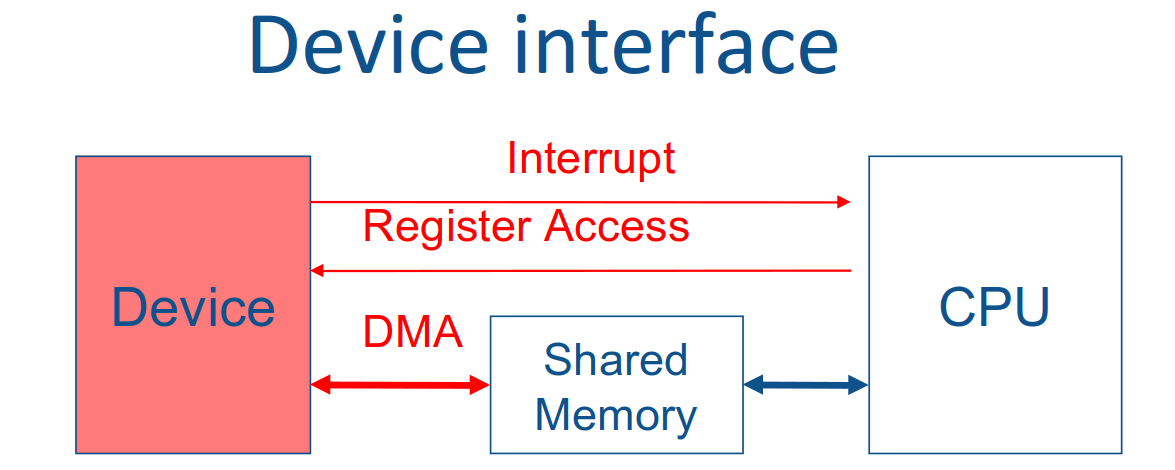
\includegraphics[width=1.\textwidth]{device-interface}
			
		\end{column}
		
		\begin{column}{.6\textwidth}
			
		\begin{itemize}
			\item Interaction between device and driver:
			\begin{itemize}
				\item Driver programs device through register access 
				\item Device notifies driver through interrupt
				\item Device could DMA for massive data movement
				
			\end{itemize} 
		
	  \end{itemize} 	
			
			
		\end{column}
		
		
	\end{columns}
	
	
\end{frame}


%-------------------------------------------------
\begin{frame}
	\frametitle{Device Interface in VMM}
	
	
	
	\begin{columns}
		
		\begin{column}{.4\textwidth}
			\centering
			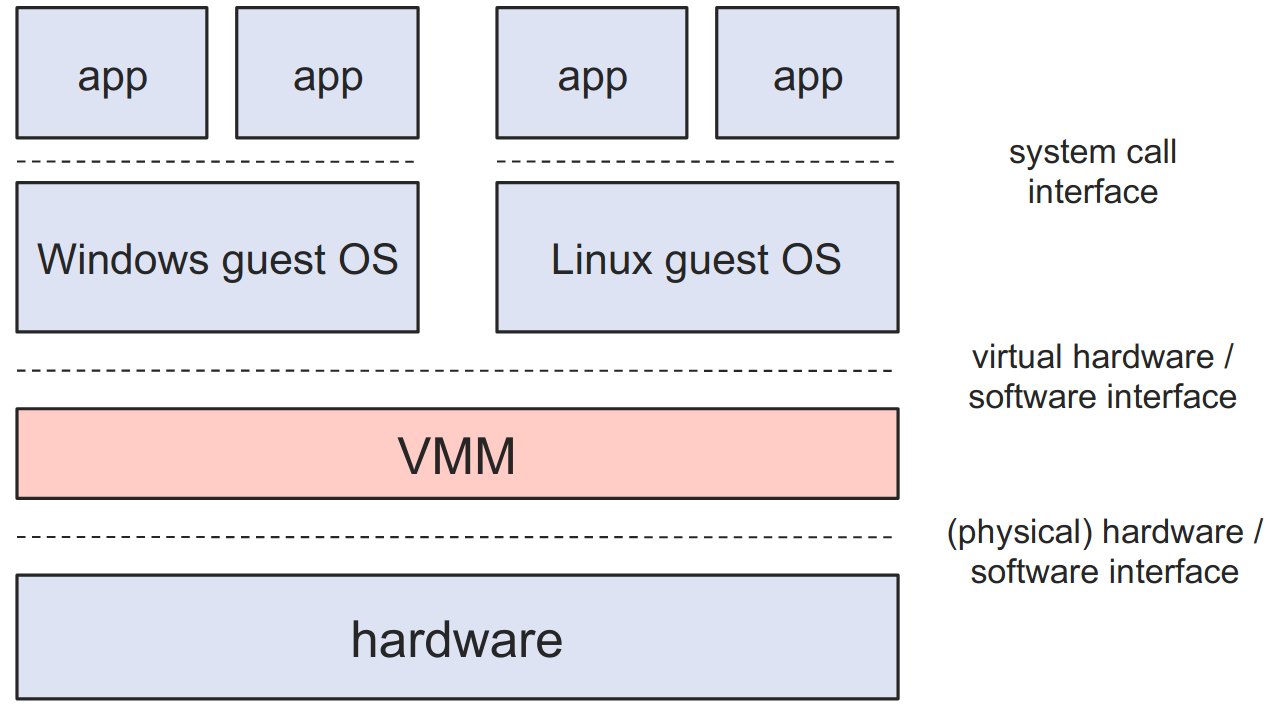
\includegraphics[width=1.\textwidth]{vmm-do-work}
			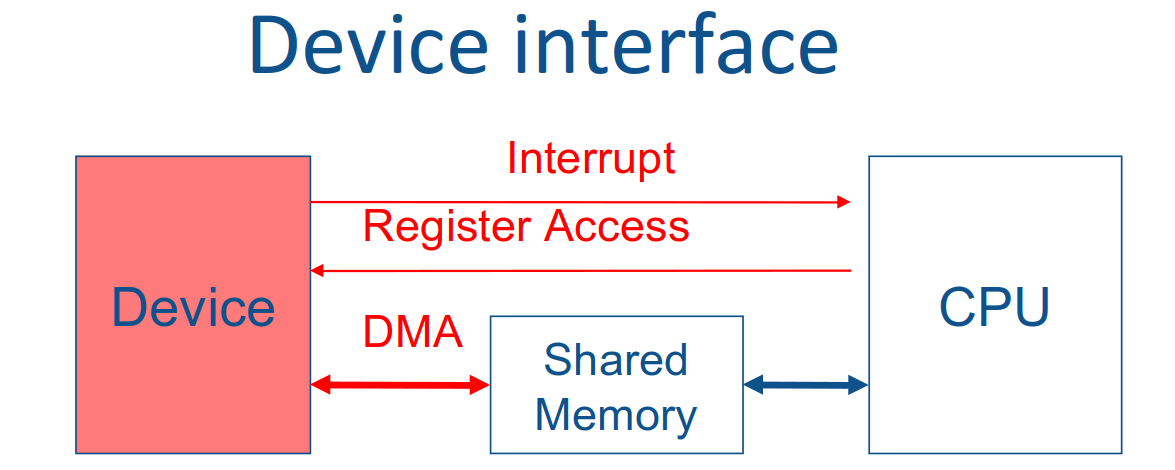
\includegraphics[width=1.\textwidth]{device-interface}
		\end{column}
		
		\begin{column}{.6\textwidth}
			
			\begin{itemize}
				\item I/O Virtualization requires the hypervisor to present guest a complete device interface
				\begin{itemize}
					\item Presenting an existing interface
    				\begin{itemize}
    					\item  {\color{blue}Software Emulation}
    					\item  {\color{blue}Direct assignment}
    				\end{itemize} 
					
				\item Presenting a brand new interface
				\begin{itemize}
					\item {\color{blue}Paravirtualization}
					
				\end{itemize} 
				\end{itemize} 
			\end{itemize} 	
			
			
		\end{column}
		
		
	\end{columns}
	
	
\end{frame}

%-------------------------------------------------
\begin{frame}
	\frametitle{I/O Software Emulation in VMM}
	
	
	
	\begin{columns}
		
		\begin{column}{.4\textwidth}
			\centering
			%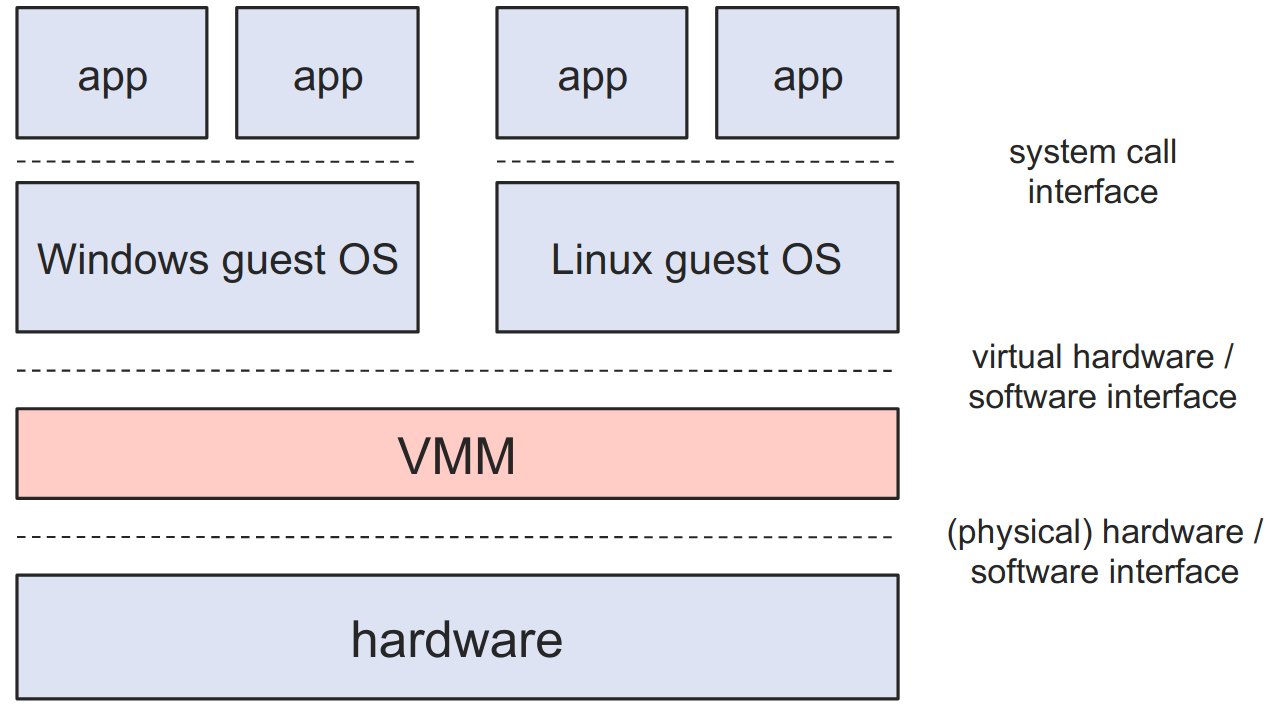
\includegraphics[width=.8\textwidth]{vmm-do-work}
			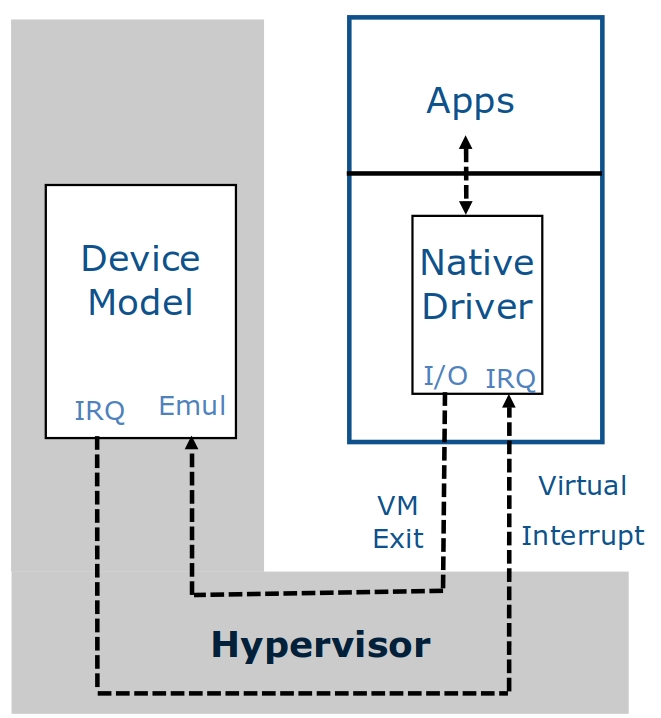
\includegraphics[width=.9\textwidth]{vmm-io-soft-emulation}
		\end{column}
		
		\begin{column}{.6\textwidth}
			%Software Emulation
			\begin{itemize}
				\item Guest runs native device driver, e.g. NE2000
				\begin{itemize}
					\item I/O access is trap-and-emulated by device model in hypervisor
					\item Translation for MMIO is zapped
					\item Virtual Interrupt is signaled by device model per semantics
					
				\end{itemize} 
				\item Excessive trap and emulation

			\end{itemize} 	
			
			
		\end{column}
		
		
	\end{columns}
	
	
\end{frame}

%-------------------------------------------------
\begin{frame}
	\frametitle{Paravirtualization}
	
	
	
	\begin{columns}
		
		\begin{column}{.4\textwidth}
			\centering
			%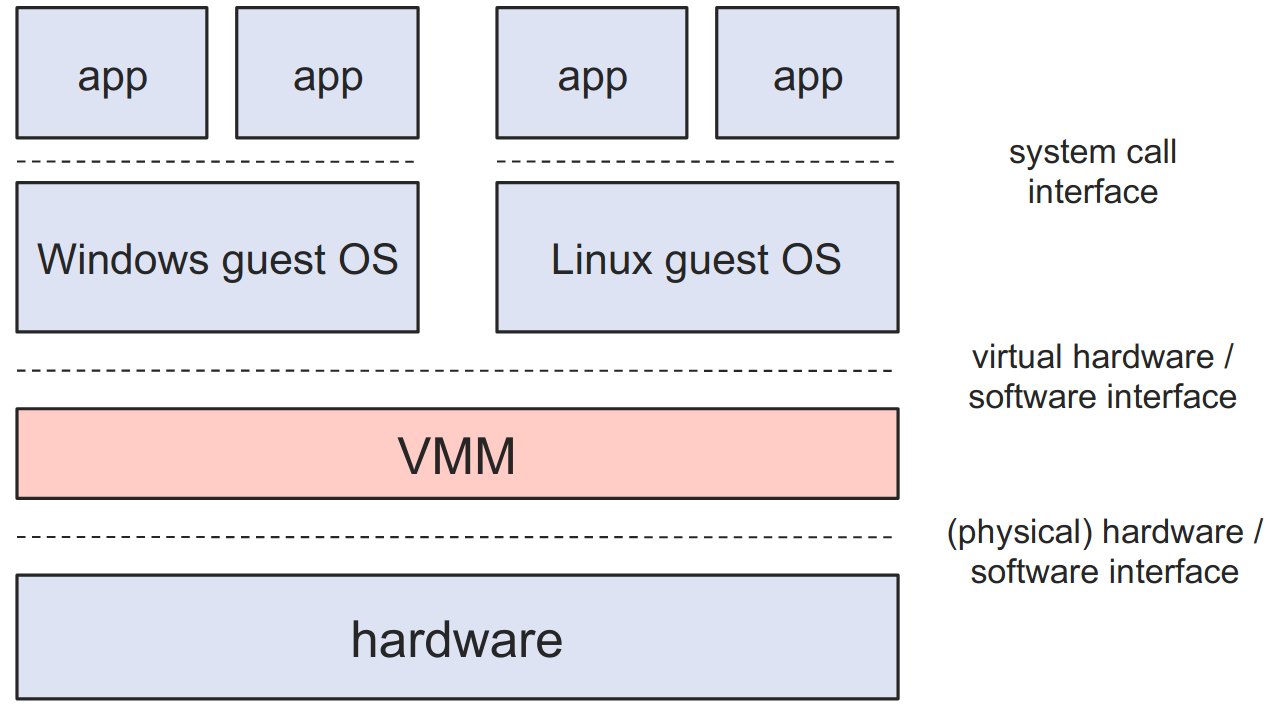
\includegraphics[width=.8\textwidth]{vmm-do-work}
			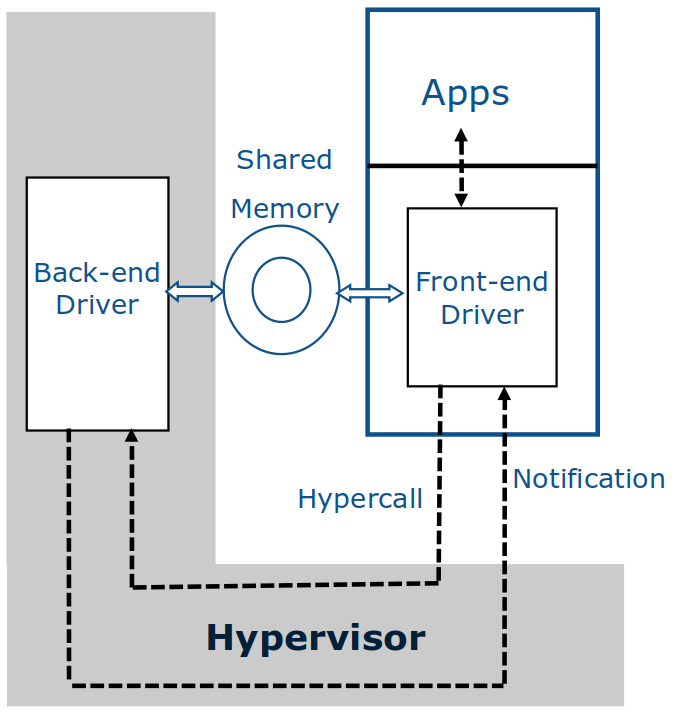
\includegraphics[width=.9\textwidth]{vmm-io-paravirt}
		\end{column}
		
		\begin{column}{.6\textwidth}
			%Paravirtualization
			\begin{itemize}
				\item A new front-end driver (FE driver) is run in guest
				\begin{itemize}
					\item Optimized request through hypercall
					
				\end{itemize} 
			
				\item Hypervisor runs a back-end driver (BE driver) to service request from FE driver
				\begin{itemize}
					\item Notify guest for processing
	
				\end{itemize} 			
			
			\item Shared memory is used for massive data communication
			\begin{itemize}
				\item To reduce guest/hypervisor boundary crossin
				\item e.g. Xen VNIF, KVM Virtio-Net
			\end{itemize} 
			
			\end{itemize} 	
			
			
		\end{column}
		
		
	\end{columns}
	
	
\end{frame}
%-------------------------------------------------
%-------------------------------------------------


\end{document}